\documentclass[11pt]{report}
\usepackage[a4paper, bmargin=2.7cm, tmargin=2cm, lmargin=2cm, rmargin=2cm]{geometry}
\setcounter{tocdepth}{1}

% Spacing stuff
\setlength{\parindent}{2em}
\setlength{\parskip}{.5em}
\renewcommand{\baselinestretch}{1.1}
\usepackage{enumitem}

\usepackage[T1]{fontenc}
\usepackage[utf8]{inputenc}

\usepackage{natbib}
\usepackage{lmodern}
\usepackage{booktabs}
\usepackage{amsthm}
\usepackage{amsmath}
\usepackage{amssymb}
\usepackage{mathrsfs}
\usepackage{physics}
\usepackage{graphicx}
\usepackage{tikz}
\usepackage{caption}
\usepackage{multirow}
\usepackage{titlesec}
\usepackage{afterpage}
\usepackage{lipsum}
\usepackage{xcolor}
\usepackage{hyperref}
\usepackage{verbatim} 
%AIMERIC ADDITIONS
\usepackage{rotating}


% Commands
\newcommand{\df}{\equiv}
\newcommand{\setas}{\overset{!}{=}}
\newcommand{\refeq}[1]{(\ref{#1})}
\newcommand{\com}[1]{\textbf{\color{red}[#1]}}
\newcommand{\with}{\quad\text{with}\quad}
\newcommand{\munu}{{\mu\nu}}
\newcommand{\smallsum}{\,\raisebox{-3pt}{\text{\LARGE $\Sigma$}}\hspace{1pt}}
\newcommand{\Msol}{M_\odot}
\newcommand{\zsp}{z_\mathrm{spec}}
\newcommand{\zph}{z_\mathrm{phot}}
\renewcommand{\AA}{\r{A}\,}
\newcommand\blankpage{%
    \null
    \thispagestyle{empty}%
    \addtocounter{page}{-1}%
    \newpage}

% Sections renewal
\newcommand{\theromanchapter}{\Roman{chapter}}
\titleformat{\chapter}{\huge\bfseries}{\theromanchapter\;--}{6pt}{}
\titlespacing{\chapter}{0pt}{20pt}{15pt}
\titlespacing{\section}{10pt}{10pt}{10pt}
\titlespacing{\subsection}{20pt}{10pt}{10pt}




\begin{document}

% Title Page
\thispagestyle{empty}
\begin{center}
    \centering
  % logos
    
\includegraphics[height=45pt]{fig/logo_cnrs.jpg}\hspace{30pt}
    
\includegraphics[height=65pt]{fig/Logo_Phelma.png}\hspace{30pt}
    
\includegraphics[height=65pt]{fig/logo_uga_vo_cmjn.jpg}\hspace{30pt}
    
\includegraphics[height=55pt]{fig/logo_cppm.png}\par
    \vspace{1cm}
  % Head
    {\large Université Grenoble Alpes -- Second year Masters degree \\ [3pt] \textsc{Physique subatomique et cosmologie}\par}
    {\large Grenoble INP Phelma \\ [3pt] \textsc{Physique, Nanosciences}\par}
    \vspace{8pt}
    {\ - \par}
    \vspace{8pt}
    {\large Centre de Physique des Particules de Marseille\par}
    \vspace{12pt}
  % Title
    \rule{\linewidth}{1pt}\par
    \vspace{2pt}
    \LARGE{\textsc{Neutrino Mass Hierarchy Measurement \\[2pt] Particle Identification using Neural Networks}}
    \rule{\linewidth}{1pt}\par
    \vspace{10pt}
  % Names
    {\Large Aimeric \textsc{Landou}\par}
    \vspace{12pt}
    {\Large \textsc{Supervisor:} \\[4pt] \large Dr. Paschal \textsc{Coyle}  (CPPM)\\coyle@cppm.in2p3.fr \par}
    \vspace{8pt}
    {\Large \textsc{Phelma Tutor:} \\[4pt] \large M. Lionel \textsc{Bastard} \\bastard@minatec.grenoble-inp.fr\par}
    \vspace{8pt}
    {\Large \textsc{UGA Tutor:} \\[4pt] \large Dr. Aurélien \textsc{Barrau}\\barrau@lpsc.in2p3.fr\par}
    \vspace{18pt}
\end{center}
  % Date
\begin{center}
\vspace{20pt}
    {\large from 05/03/2018 to 28/07/2018}
\end{center}



\tableofcontents

\chapter*{Glossary:}

{\Large
\begin{itemize}
\item NMH - Neutrino Mass Hierarchy
\item NN - Neural Network
\item TMVA - Toolkit for Multivariate Data Analysis
\item PID - Particle Identification
\item CC - charged current 
\item NC - neutral current
\item DOM - Digital Optical Module
\item PMT - Photomultiplier
\end{itemize}
}

\listoffigures

\chapter*{Introduction}
\addcontentsline{toc}{chapter}{Introduction}




In 2015, the Nobel Prize in Physics has been awarded to T. Kajita and A. B. McDonald, for "the discovery of neutrino oscillations, which shows that neutrinos have mass". For forty years, a discrepancy had been observed between the expected flux of neutrinos from the Sun and the flux measured. The model of neutrino oscillation imagined by B. Pontecorvo in 1957 was one of the many models trying to explain this discrepancy at the time. This model predicts that neutrinos can change their nature, in fact their flavour, as they travel over large distances. This phenomenon though has one important implication: for them to oscillate, neutrinos must have a mass, different for each of the three states, something that goes against the prediction of the Standard Model, which says their mass should be zero. This question remains, as of today, unanswered.

Most of the parameters involved in the neutrino oscillations have been measured in the last decades. One of the remaining unknowns is the question of the Neutrino Mass Hierarchy. Only two absolute mass differences have been measured between out of the three states. Which of the two possible solutions, the Normal Hierarchy or the Inverted Hierarchy, is the right one is still an open question. Answering the question of the Neutrino Mass Hierarchy is one of the main missions of the KM3NeT collaboration, in charge of ORCA. Built on the sea-floor of the Mediterranean Sea, ORCA is a Cherenkov neutrino telescope, that records in his kilometric volume the light emitted by charged secondary particles created during the interaction of a neutrino with the surrounding water. 

One of the critical steps in the Neutrino Mass Hierarchy measurement is the identification of the flavour of the detected neutrinos. If the current tools used to discriminate between the different flavours -- a machine learning algorithm called Random Decision Forest -- performs well at the high-end of the energy range seen by ORCA, the performance achieved at the lower edge (1--10 GeV) is relatively poor. Besides, this algorithm uses brute force to classify the events by using all of the near two hundred variables reconstructed from the raw data of the detector. The goal of this study is to improve the particle identification at these energies by using a different kind of machine learning algorithm -- a Neural Network -- and to reduce the number of variables necessary to the classification.

We will first introduce the background and tools necessary to the understanding of the study. Then we will present the performance of the Neural Network and compare it to the current Random Decision Forest.



\chapter{Theoretical Context}\label{Theoretical_Context}
\section{Neutrinos}

Around $10^{15}$ of these elusive and mysterious particles traverse our body every second citep{Bahcall:2004pz}
%https://arxiv.org/pdf/astro-ph/0412440.pdf ; Bahcall, John N.; Serenelli, Aldo M.; Basu, Sarbani (2005). "New Solar Opacities, Abundances, Helioseismology, and Neutrino Fluxes". The Astrophysical Journal. 621 (1): L85–8. arXiv:astro-ph/0412440 Freely accessible
, and yet we discovered these ghosts only relatively recently. Different experiments finally allowed us to see them, or rather see their interaction with other particles, and to start measuring their various characteristics and properties. 1956 saw the first proof of their existence \citep{Cowan:1992xc}, 22 years after Pauli had first written his idea of the neutrino in a paper \citep{Brown:1978pb}. A different type of neutrino is discovered 6 years later \citep{Danby:1962nd} in 1962: with the last kind discovered in 2000 \citep{Kodama:2000mp}, the three classes of neutrinos, or flavours, will  be named electron, muon and tau neutrino. While their oscillation is already being theorised in the 60's, due to the Solar neutrino problem -- a missing number of neutrinos detected in a previous experiment -- these oscillations have only been observed in 2001, with the Sudbury Neutrino Observatory \citep{Ahmad:2002jz}. Although they were first thought massless, these oscillations brought the proof of a non-zero mass. A lot of questions remain today. In particular, we only have measured two absolute squared-mass differences among the three kinds of neutrinos, and thus don't know the full mass ordering. This is the Neutrino Mass Hierarchy problem.

\subsection{What is a neutrino?}
Neutrinos are almost massless elementary particles with half-integer spin - they are thus fermions -- and no electric or colour charge. Because of that, they can only interact through the Weak Interaction -- from this come their elusive nature.

There are three flavour of neutrinos known so far: electron neutrino ($\nu_{e}$), muon neutrino ($\nu_{\mu}$) and tau neutrino ($\nu_{\tau}$), each one associated to his lepton counterpart, electron, muon and tau. These flavours are called interaction eigenstates: they are the quantum states that we can detect, and in which neutrinos are created or projected onto during a flavour interaction (through charged current, CC, with the exchange of a $W^+$ or $W^-$ boson, or neutral current, NC, through the exchange of a Z boson). However, they are not the eigenstates of the Hamiltonian (or mass eigenstates). Thus, during the propagation of the particle, the different components projected onto the mass eigenstates basis evolve on their own, and the mixing happens. The mass eigenstates of the neutrino are called ($\nu_{1}$), ($\nu_{2}$) and ($\nu_{3}$). Eq. \refeq{LJFESUIH} describes the decomposition of a neutrino created in an interaction eigenstate onto the three mass eigenstates, and Eq. \refeq{ESFNIMNFU} describes the mixing that occurs during the propagation of this same neutrino.

\begin{equation}
    {\ket{\nu (t=0)}= \ket{\nu_\alpha} = \sum_{k=1}^{3}{U_{\alpha k} ^{*} \ket{\nu_k}}} 
    \label{LJFESUIH}   
\end{equation}
where $\nu_\alpha = \nu_e, \nu_\mu$ or $\nu_\tau$ and $U_{\alpha k} ^{*}$ is a coefficient of the conjugate of the unitary neutrino mixing matrix, often called PMNS matrix \citep{Patrignani:2016xqp}.

\begin{equation}
    {\ket{\nu (t)} = \sum_{k=1}^{3}{U_{\alpha k} ^{*} exp(-i(E_k t - \mathbf{p_k} \cdot \mathbf{x})) \ket{\nu_k}}}
    \label{ESFNIMNFU}
\end{equation}
where $E_k$ is the energy of the neutrino, $\mathbf{p_k}$ its momentum and $\mathbf{x}$ its position. 

\subsection{Neutrino Mass Hierarchy}

One can show that the oscillation probability between two flavours in the vacuum is directly proportional to the squared sine of the absolute mass squared differences \citep{Zuber:2004nz}. In a two-flavour case, this can be written as in Eq. \refeq{AOZIEJ}:

\begin{equation}
    {P_{\alpha \beta}} \propto \sin ^2 \left(\frac{{\Delta m}_{21} ^2*L}{4E_\nu}\right)
    \label{AOZIEJ}
\end{equation}
where:
$|{\Delta m}_{21} ^2|=|{m_2 ^2-m_1 ^2}|$ and ${P_{\alpha \beta}}$ is the probability for a neutrino of flavour $\alpha$ to oscillate into the flavour $\beta$.

Two absolute mass-squared differences have been measured so far, one thanks to the neutrinos from the sun, and the other thanks to atmospheric neutrino \citep{Patrignani:2016xqp}. 

We only know 2 absolute squared-mass differences because the functions involved in theses oscillation probabilities are even (see Eq. \refeq{AOZIEJ}). Previous studies have reduced the number of possible orderings to two: the normal hierarchy (NH) and the inverted hierarchy (IH), only set apart by one sign in the mass differences. This is schematised in Fig. \ref{fig:POAZFN}. The convention is to name $\nu_1$ and $\nu_2$ the two mass eigenstates measured by the sun experiment, with $\nu_1$ being the lighter state, and $\nu_3$ the last state, which squared-mass difference with $\nu_2$ has been measured by looking at atmospheric neutrinos.

\begin{figure}[h!]
    \centering
    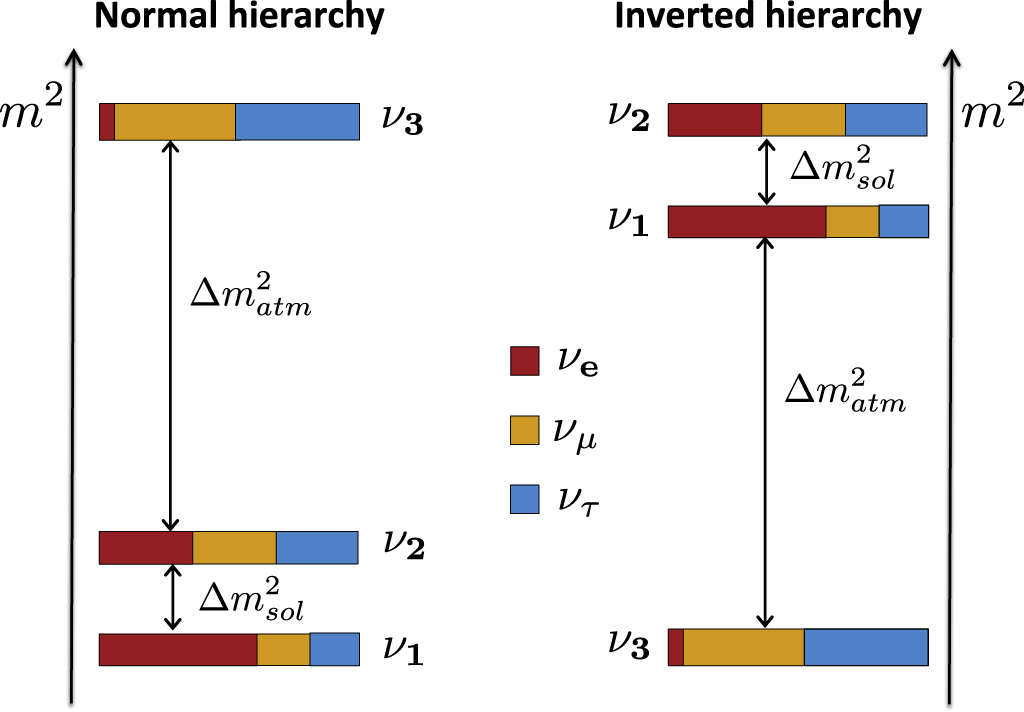
\includegraphics[width=0.60\textwidth]{fig/Neutrino_mass_hierarchy_LoI.jpg}
    \caption{Schematic illustration of the two distinct neutrino mass hierarchies. The colour code indicates the flavour composition ($\nu_e$, $\nu_\mu$, $\nu_\tau$) in each mass eigenstates ($\nu_1$, $\nu_2$, $\nu_3$). From \citep{Hofestaedt2017}}
    \label{fig:POAZFN}
\end{figure}

To decide on the right solution, ORCA makes use of the effective potential encountered by the neutrinos coming from the other side of the Earth during their propagation through its mantle and core. This effective potential mainly impacts electron neutrino events as it originates from the interaction of electron neutrinos with the electrons in matter, and breaks the evenness of the oscillation probability, allowing us to get a signed squared-mass difference.

For the measurement the detected neutrinos are characterised by flavour, energy and direction (length traveled through the Earth) and the obtained distributions are compared with the expectations from the two different hypotheses: NH, IH. These expectations are represented in Fig. \ref{fig:AIOJZOJ} for the muon flavour, in the Energy-Azimuth Angle plane, and by using true quantities, i.e with a infinite resolution and no error on the energy and azimuth angle. The asymmetry is larger in the bottom left part of both plots. The asymmetry can be defined as a function A with the formula $A=\frac{N_{NH}-N_{IH}}{N_{NH}}$, where $N_{NH}$ and $N_{IH}$ are the number of expected events for the normal hierarchy and the inverted hierarchy , and can be plotted to get a better idea of the amplitude of the change. This is done in Fig. \ref{fig:JUHDNB} after applying a smearing to simulate the finite precision of the detector. To the left the plot is done for electron neutrinos and antineutrinos, and to the right for muon neutrinos and antineutrinos. Again, the largest asymmetry value can be found at low energy, between 1 and 10 GeV. This is where the study will focus on for the classification comparison.

\begin{figure}[h!]
    \centering
    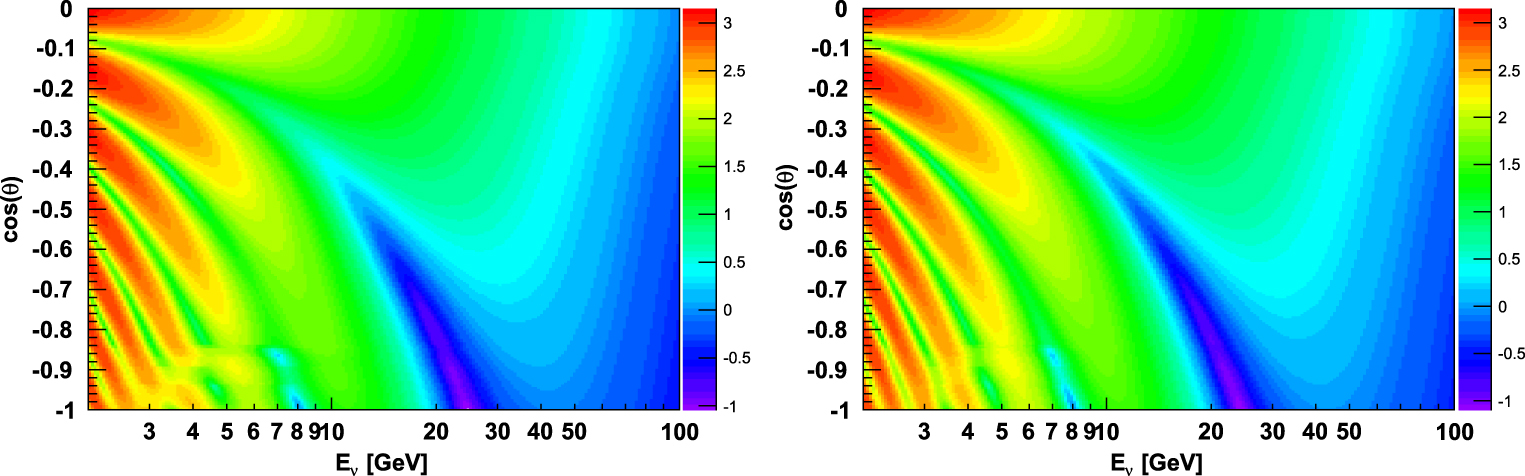
\includegraphics[width=0.90\textwidth]{fig/numu_IH_vs_NH.jpg}
    \caption{
    $\nu_\mu + \nu_\mu$ event rate (units of $GeV^{-1}y^{-1}s^{-1}$ in log scale) as a function of the neutrino energy and cosine of the zenith angle, for a 1 Mton target volume. The left (right) plot shows the distribution for the normal (inverted) mass hierarchy. From \citep{Adrian-Martinez:2016fdl}}
    \label{fig:AIOJZOJ}
\end{figure}

\begin{figure}[h!]
    \centering
    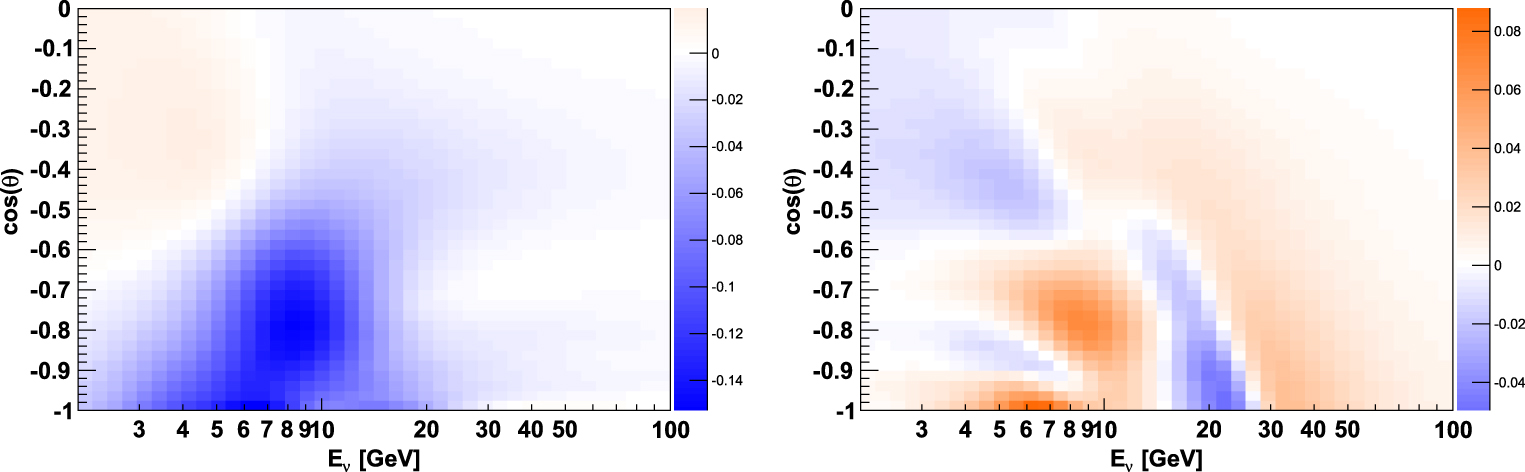
\includegraphics[width=0.90\textwidth]{fig/numu_vs_nue_Asymmetry.jpg}
    \caption{Asymmetry between the number of $\nu +\bar{\nu }$ CC interactions expected in case of NH and IH, expressed as a function of the energy and the cosine of the zenith angle. The right (left) plot applies to muon (electron) neutrinos. A smearing is applied on the energy and on the azimuth angle to simulate the resolution of the detector. From \citep{Adrian-Martinez:2016fdl}}
    \label{fig:JUHDNB}
\end{figure}

\subsection{KM3NeT/ORCA}

KM3NeT/ORCA is one of the two neutrino detectors being built inside the KM3NeT collaboration (its counterpart, being built in Italy, is named ARCA). ORCA is a kilo-metric lattice of Digital Optical Modules (DOMs) being installed at the bottom of the Mediterranean Sea, that will eventually be arranged in 115 strings (or lines) of 18 DOMs each, spaced by 9 meters \citep{Adrian-Martinez:2016fdl}. In each DOM, 31 photomultipliers (PMTs) looking covering roughly every directions recover the Cherenkov light emitted in a cone along its path by the charged secondary particles produced in a neutrino interaction, as they propagate through the water\footnote{The Cherenkov phenomenon appears when a charged particle propagates in a medium above the phase velocity of light in this medium. It manifests as a cone of light being emitted along the path of the particle.}. The disposition of the DOMs has been designed to allow the detection of neutrinos in the few-GeV energy range (compared to TeV energy scale for ARCA in Italy) \citep{Adrian-Martinez:2016fdl}.

At high energy, the two main kinds of events (also the ones studied in this report) are easily recognisable. A muon produced by CC muon-neutrino interaction propagating through the detector appears once reconstructed as a straight line, while NC events and CC tau and electron-neutrino events emit a shower of secondary particles that tend to appear as point like in the detector in the low-energy range of 1--10 GeV, the spatial dimensions being too small compared to the spacing of the DOMs \citep{Adrian-Martinez:2016fdl}. Fig. \ref{fig:POJRIDG} shows the two typical patterns. The shower-like events on the right seems to have been induced by a high energy neutrino as the shower pattern can clearly be seen.

\begin{figure}[h!]
    \centering
    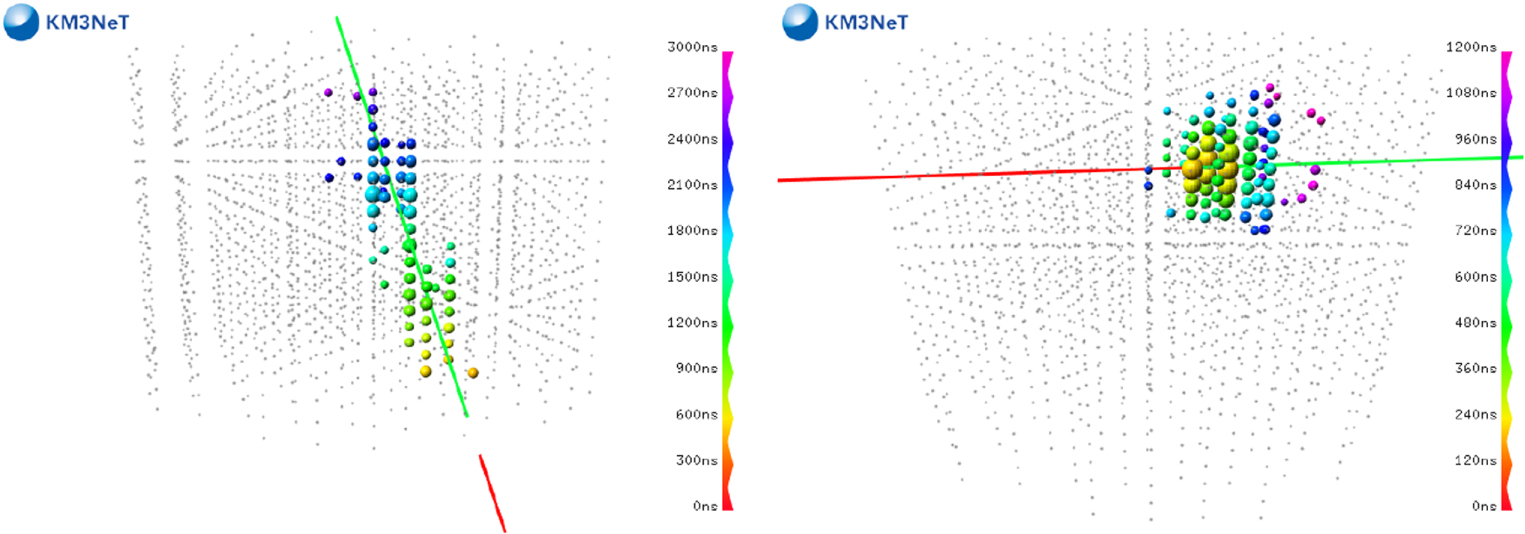
\includegraphics[width=0.90\textwidth]{fig/Shower_vs_Track.jpg}
    \caption{Event displays for a simulated ${\nu }_{\mu }$ CC event (left) and a contained ${\nu }_{\mu }$ NC event (right). The incoming neutrinos are indicated by the red line, and the outgoing lepton by the green line. The colour scale gives the hit times with respect to the time of the neutrino interaction. DOMs without hits are shown by grey dots. From \citep{Adrian-Martinez:2016fdl}}
    \label{fig:POJRIDG}
\end{figure}

Finally, such a detector built close to the sea level would be unable to detect any neutrino. Or rather, we would be unable to distinguish the rare events from the bulk that would be produced by the constant bombardment by atmospheric muons, created in the atmosphere by the collision of cosmic rays with particles of the atmosphere. Even at around 2450 meters below the surface though, the rate of atmospheric muons of the right energy range reaching the detector is about $10^5$ orders of magnitude higher than the rate of neutrinos in the GeV energy-scale citep{Hofestaedt201}. A way of greatly reducing this difference is looking at up-going neutrinos having been created on the other side of Earth, as muons cannot traverse the Earth.

\section{Particle Identification: PID}

The track and shower patterns are easily recognisable, most of the time. However, at low energy (1 to 10 GeV, where we are most sensitive to the NMH) a track is often too small compared to the resolution of the detector and thus is reconstructed as point-like, a signature characteristic of showers. Unfortunately, no magic variable built from the data recorded for one event has yet been found on which a cut would result on a good discrimination power at these energies.

The measurement of the Neutrino Mass Hierarchy as presented previously asks for a way of discriminating electron neutrinos from muon neutrinos. Unfortunately, no magic variable built from the data recorded for one event has yet been found on which a cut would result on a good discrimination power. That is where machine learning can play a role. By being trained on a large set of data, a machine learning algorithm can discern patterns in a multi-dimensional space. One of machine learning’s many applications is non-linear classification of large volumes of data. That is, recognise whether one data point belongs to one predefined class or another. The main difference between a linear classifier and a non-linear one is summarised in Fig. \ref{fig:NUIO} in a 2-dimensional case: a non-linear classifier can simply divide a plane using contours different from a line. These two examples, although quite simple with only two variables, give a visual idea of what a machine learning algorithm does. Only, they can work on multiple-dimensional data.

\begin{figure}[h!]
    \centering
    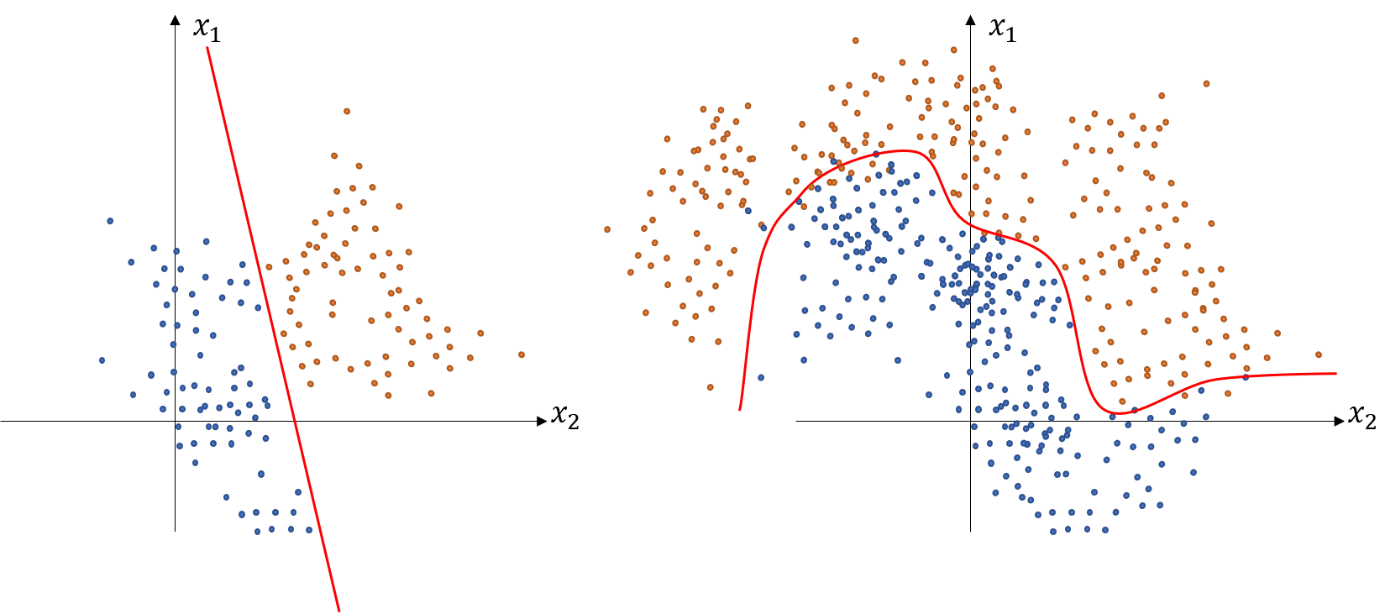
\includegraphics[width=0.8\textwidth]{fig/Classification_2D_comparison.png}
    \caption{Schematic representation of the classification in 2 dimensions for a linear classifier on the left and a non-linear classifier on the right.}
    \label{fig:NUIO}
\end{figure}

With around 200 variables reconstructed from the raw data for one single event for KM3NeT, the number of dimensions is far too large for a human to be able to find patterns. A kind of machine learning algorithm called Random Decision Forest has been used until now to navigate through this data, working on all the variables available.

\subsection{Random Decision Forest}

Lots of different machine learning algorithms exist. The one used for this PID at the moment is a Random Decision Forest algorithm (RDF). A Random Decision Forest is composed of many trees (the algorithm used in the PID has 101 of them), each trained independently and making his own assumption. Then user can then decide on the number of trees he wants to agree with each other to make a decision -- here we simply decide based on the majority.

A tree is built recursively. Once he’s given a set of data divided into two classes (0 and 1), he will find the variable that gives the best separation between the two classes, make a cut, and save the value and the name of the variable in a first node. For each side of the cut, the algorithm will do the exact same thing, and continue to do so at each new node until a stop condition is met. While asking the algorithm to stop when the samples at the output of a node are composed of only one class would give the best results for the training dataset, this kind of condition would lead to an obvious overtraining, where the tool has learned details of the noise in the training data and will behave poorly when given new data: this is the Bias-Variance trade-off \citep{hastie_09_elements-of.statistical-learning}. Thus, more elaborate stop conditions are usually used, to counter this effect.

The reason for this work was to reduce the number of variables used, and try to improve the classification for low energy neutrino events: too many variables might indeed be messing with the current training. Another machine learning algorithm has been chosen for that: a neural network.
    
\subsection{Neural Network}

\subsubsection{What is a Neural Network?}

\qquad A neural network, or NN, is a non-linear mathematical function, transforming an input into its image, represented by a collection of nodes, or neurons, ordered in layers, and linked together \citep{MacKay2003}. A very simple network is presented in Fig. \ref{fig:XXX}. An event injected in the first layer, or input layer, in the form of an array of numbers see its information propagate through the network and undergo transformations until it reaches the last layer, or output layer. The layers between the first and the last ones are called hidden layers.

\begin{figure}[h!]
    \centering
    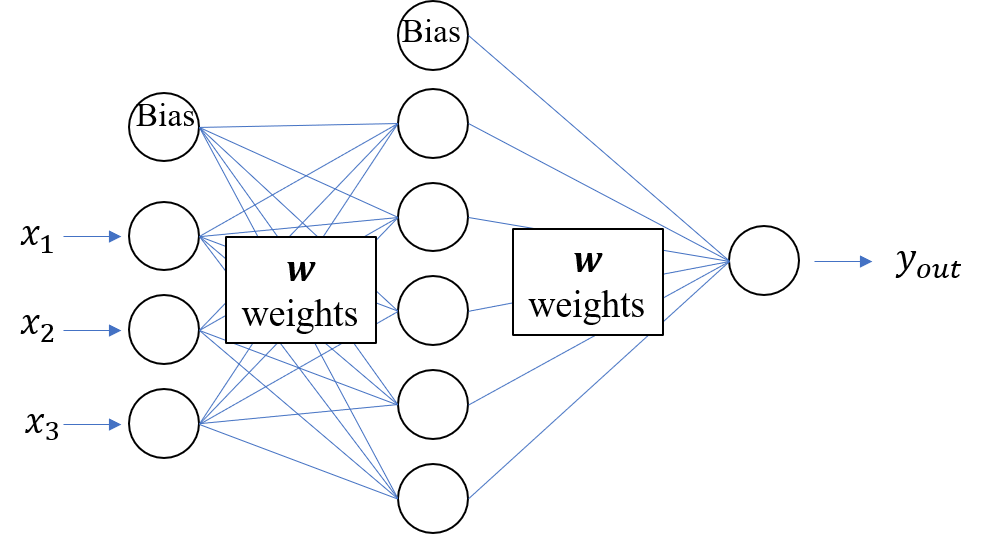
\includegraphics[width=0.65\textwidth]{fig/NN_shape_et_layout.png}
    \caption{Representation of a neural network with 3 input neurons, 1 hidden layer and 1 output neuron.}
    \label{fig:XXX}
\end{figure}

For each input event $X_a$ = ($x_1$, $x_2$, …, $x_n$), and for a set of weights w, we have an image $y_{out}$($X_a$), which in our case is a real number and the verdict of our neural network on the classification of this event. We can see the transformation of this event as the network processing a signal. Let’s look at how this signal propagates from one layer to the next. The neurons of the first layers each receive one the n variables describing the event $X_a$ and directly transmit it without transformation. The transformations take place on the other layers. Each neuron of one of these layers, hidden layers and output layer, receive as an input the output of all the neurons of the previous layer multiplied by the weight of the corresponding connexion. These inputs then undergo a transformation that can be divided into two functions. First, a synapse function – in our case a simple sum – projects this multidimensional input onto one one-dimensional variable, that then goes through the neuron activation function, a non-linear function – in our case the hyperbolic tangent function. The non-linearity of this function is necessary to get a good classification of complex non-linear structures. This structure is summarised in Figure \ref{fig:ZERAZE}, and Eq. \refeq{AQSD} shows the output of the first neuron of the (i+1)-th layer as a function of the outputs of the neurons of the i-th layer.

\begin{figure}[h!]
    \centering    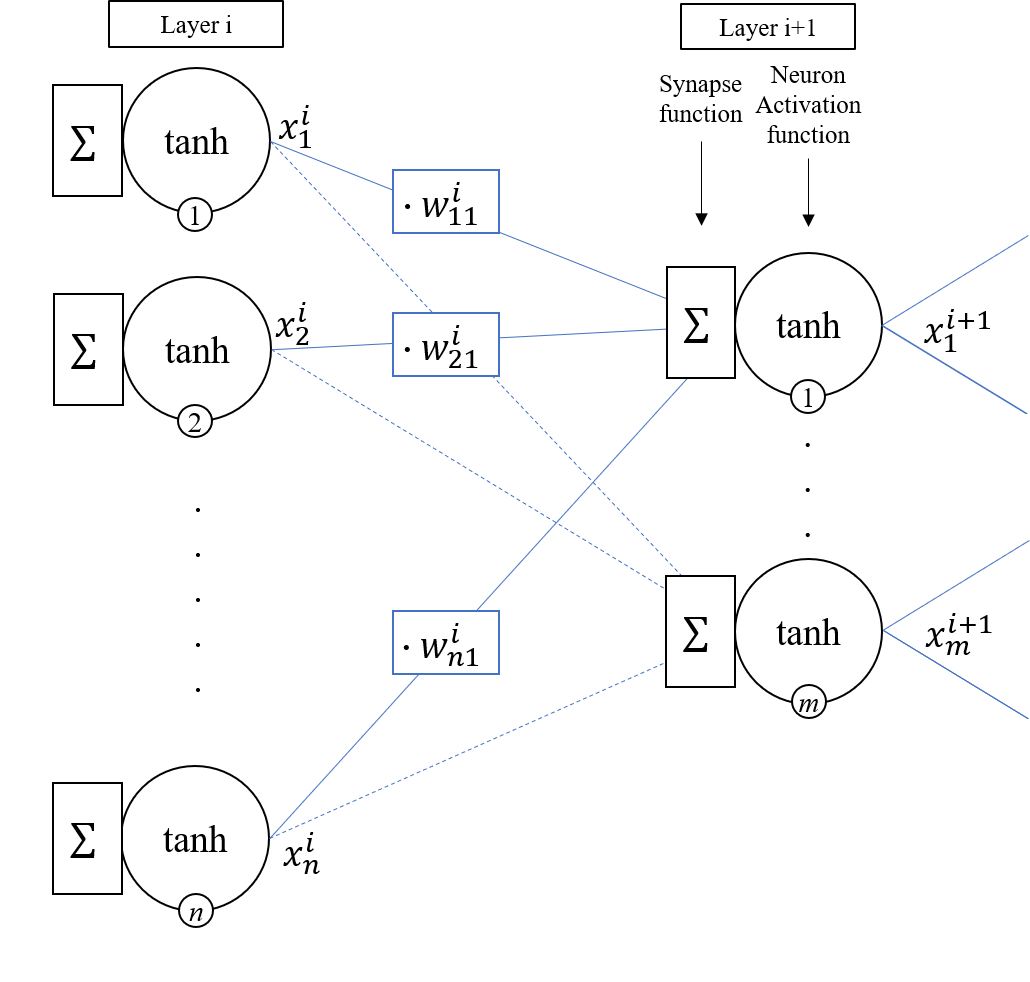
\includegraphics[width=0.65\textwidth]{fig/NN_activation_et_synapse.png}
    \caption{
    Schematic representation of the interface between two layers. $x_i ^j$ is the output of the j-th neuron of the i-th layer.}
    \label{fig:ZERAZE}
\end{figure}

\begin{equation}
    {x_1}^{i+1} = \tanh \left(\sum_{k=1}^{n}{x_k ^{i}w_{k,1}^{i}} \right) \dot{}
    \label{AQSD}
\end{equation}

 In each layer a Bias node is present. Its output is independent of the outputs of the previous layer, often set to 1, and its impact, dictated by the weights of its connexions, is only modified during the training. Such a neuron introduces an affine shift in the inputs of the following layer it is connected to, and contributes to the non-linearity of the model.

\subsubsection{Back Propagation}

\qquad The training consists in finding the right weights for the task considered. To train the network, we feed it events from a set of data similar to the one we want it to later be able to classify automatically – the training dataset being either real data or, in our case, simulated data, for which we’re able to distinguish both categories. The network’s answer $y_{out}$($X_a$) of each event $X_a$ is compared to the image of this event by the expected value function $\hat{y_a}$$\in$[0,1]. This function $\hat{y_a}$ maps a class\_0 event onto 0, and a class\_1 event onto 1. Note that this is a choice well suited to our problem, featuring only two classes, but we could have chosen a different set of values and it wouldn’t have had any impact. This comparison is done through the introduction of an error function e (Eq. \refeq{YYaYeYwY}) measuring the quadratic deviation of the network’s output to this expected value.

\begin{equation}
    e(X_a|w) = \left(y_{out}(X_a)-\hat{y_a}\right)^2
    \label{Tmunu}
\end{equation}
where:
\begin{equation}
    \hat{y_a} = \left\{
    	\begin{array}{ll}
			1 (class\_0) \\
            0 (class\_1)
    	\end{array}
   	\right.
    \label{YYaYeYwY}
\end{equation}

This error function holds for one set of weights, and will thus evolve during the training as the weights are re-computed. 

The deviations of all the N training events are summarised in a global error function E, characterising the answer of the network to the whole training set rather than to one single event. This global error function is defined in Eq. \refeq{wHyeuUUUUU}, and is simply the square of the Euclidian norm:

\begin{equation}
    E(X_1, X_2, ..., X_N|w) = \sum_{a=1}^{N}{e(X_a|w)} = \sum_{a=1}^{N}{\left(y_{out}(X_a)-\hat{y_a}\right)^2}
    \label{wHyeuUUUUU}
\end{equation}

To understand why we’re introducing a measurement of distance it is important to see that what we are trying to do is to build a mathematic function of a n-dimensional space (the n input variables) to a 1-dimensional space (the output of the neural network) as a generalisation of $\hat{y_a}$, which is only defined within the dataset used for the training and doesn’t look at these n variables. Ideally, this new function $y_{out}$ perfectly matches $\hat{y_a}$ on the subset of this new n-dimensional space that is the training dataset, and generalises well what it learned through the training. Unfortunately, outside of trivial classifications, these two things are often incompatible. A close to perfect match is often a hint of overtraining.

Now this global error function has been defined, the problem becomes a simple optimisation problem. We now look at E as a function of the weights $w_{k,j} ^i$, with a fixed dataset of N events, and try to get the best minimum we can find in a reasonable amount of time (assuming a minimum does exist). A common method of minimisation, and the one used by our algorithm, although not the most efficient, is the method of gradient descent. Starting from a random set of weights $w_{k,j} ^i$, the algorithm follows the direction where the opposite of the gradient of E is maximum, i.e. where E decreases most rapidly, and moves by small steps of length proportional to the gradient, the constant of proportionality being a positive number called learning rate and set by the user. The algorithm continues until the classification performance stops evolving. The training is completed.

Once a minimum has been found, the weights are saved in a file, so that the neural network can be fed new data in the future for classification.

\subsubsection{Training and testing sample}

\qquad To be able to test the trained neural network, in particular to check for overtraining, the initial data is divided into two parts. The first is the actual training sample, which will be used as described previously. What is left, called testing sample, will be classified by the neural network once the latter has been trained on the training sample. These two samples being ideally built randomly from the initial dataset, if this dataset gather a large enough number of events, they should share the same features, and the results of the classification of both samples should not be much different from one another in the absence of overtraining.

\subsubsection{Output of a neural network. Classifier distribution}
\qquad The network has been trained. How can we interpret the result of the classification of an event $X_a$ ? The only neuron of the output layer gives its answer in the form of a real number $y_{out}$$\in$[-1;1], as the image of the last hidden layer by the hyperbolic tangent function. A last transformation can be done, essentially in order to facilitate the interpretation: an affine transformation to have the final output in the range [0,1]. This output can be seen as a score characterising how close to either class the event is. The closer to 1 (0) the score, the closer the event is to class\_1 (class\_0). One now has to make a choice on how to use this result. New classes can be created based on the classifier output, by applying one or more cuts. If high purity classifications are needed, one can choose to keep only events with a classifier output close to the extrema 0 or 1, effectively applying two cuts and thus creating three classes: classified\_as\_0, classified\_as\_1 and a new unclear\_class corresponding to the middle of the classifier distribution. The purity in the meaningful classes will be high, but that will come at the expense of the amount of events effectively classified, as a lot of them with classifier outputs in the middle are discarded. On the other hand, if the amount of events is valuable, one can loosen the selection and apply only one cut in the middle of the distribution, though the purity of the two new classes will be lowered.

A qualitative evaluation of a neural network used as a classifier can be done by looking at a histogram such as the example presented in Fig. \ref{fig:ALELUIA}. For each of the two classes (class\_0 in red and class\_1 in blue), its events are given to the neural network and the outputs are collected and distributed among the bins. The two histograms are then normalised. As one could hope, class\_0 is concentrated towards 0, and class\_1 towards the value 1. Still, a non negligible amount of events have an output value in the center: the neural network hasn't been able to extract enough characteristic features. As a side note: this histogram has been plotted here for both the test sample and the training sample: in this example, one can see that both match, which is a sign that there is no overtraining here \citep{hastie_09_elements-of.statistical-learning}.


\begin{figure}[h!]
    \centering
    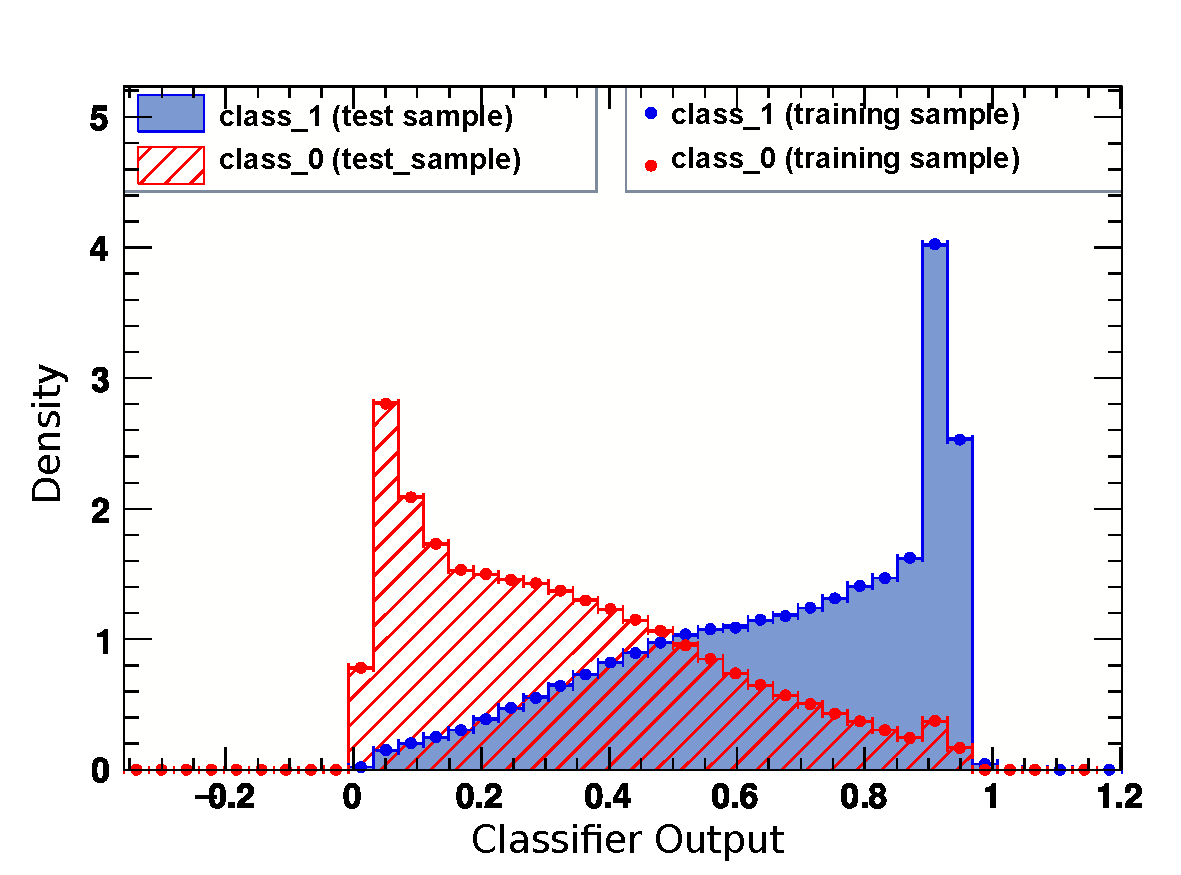
\includegraphics[width=0.55\textwidth]{fig/NN_classifier.pdf}
    \caption{Distributions of the classifier output for each class (class\_0 in red and class\_1 in blue), and each sample (dots for the training sample, full rectangles for the test sample). Each distribution is normalised to the total number of events considered.}
    \label{fig:ALELUIA}
\end{figure}

The structure of the neural network presented here is specific to the package used in this study: Toolkit for Multivariate Analysis, or TMVA \citet{2007physics...3039H}. Although the principle is the same every neural network, the specifics, such as the synapse function, the activation function or the minimisation method, can change.

This chapter introduced the different parts necessary to the understanding of the study. The next section will present the study itself.
\chapter{Classification Study} \label{Classification_Study}
The theoretical context has been set, now the study of a Neural Network as an improvement over the Random Decision Forest will be presented.

\section{Tools used}

This study follows on from years of software development inside the KM3NeT collaboration, and beyond. The data analysis in this experiment is done using the framework ROOT, which see a lot of use in particle physics, and to which new libraries proper to the collaboration are added. The neural network has been built using a ROOT package named Toolkit for Multivariate Data Analysis \citep{2007physics...3039H}, or TMVA.

The Letter of Intent shows the use of a RDF with 101 trees using close to two hundred variables reconstructed from the raw data of the detector. The neural network built is compared to this RDF.

As in the Letter of Intent \citep{Adrian-Martinez:2016fdl}, or LoI, two broad classes have been defined: "track-like" neutrino events, and "shower-like" neutrino events. The former are those induced by charged-current muon neutrino (and antineutrino) interactions, and appear in the detector as a long track. The latter are induced by all neutral current neutrino (and antineutrino) interactions, as well as charged current electron neutrino (and antineutrino) interactions, and appear in the detector as a point-like event. The two final classes, once classified by the neural network, are named "seen as track-like" and "seen as shower-like".

The dataset used in this study come in the form of a tree of 4,786,617 simulated events (Monte Carlo simulation): 1,457,943 track-like events, and 3,328,674 shower-like events, every events in this tree sharing the same data structure. Half of that is used during the training of the neural networks, and their performance are evaluated on the other half, constituting the test sample.

Thirty variables are fed to the neural network, such as the reconstructed energy, the number of PMTs hit, the total number of photons received by these PMTs, the spread of the x, y and z-distributions of hit DOMs, and many other variables built from the raw data recorded by the virtual detector during the simulation. The pool have been chosen based on the previous RDF classification, by selecting the best performing variables, and after many tries of different combinations, the best performing network has been chosen.

To compare the Neural Network and the RDF, quantities able to evaluate the classification must be defined.

\section{Useful Plots: Example of the RDF}

Two quantities have been compared: the efficiencies of the classifications and the purities of the resulting classes.

\subsection{Standard PID plot}

\qquad The LoI \citep{Adrian-Martinez:2016fdl} introduced a standard plot to evaluate the performance of the RDF classification. Shown in Fig. \ref{fig:JYVHJ}, this plot represents, as functions of the true energy of the neutrino (known because the dataset is the result of a simulation), the fraction of events identified as track-like for each class. This fraction for the track-like class is an efficiency, while for the shower-like events, the efficiency is equal to one minus the plotted fraction. This result is obtained by choosing a cut on the classifier output at 0.5.

\begin{figure}[h!]
    \centering
    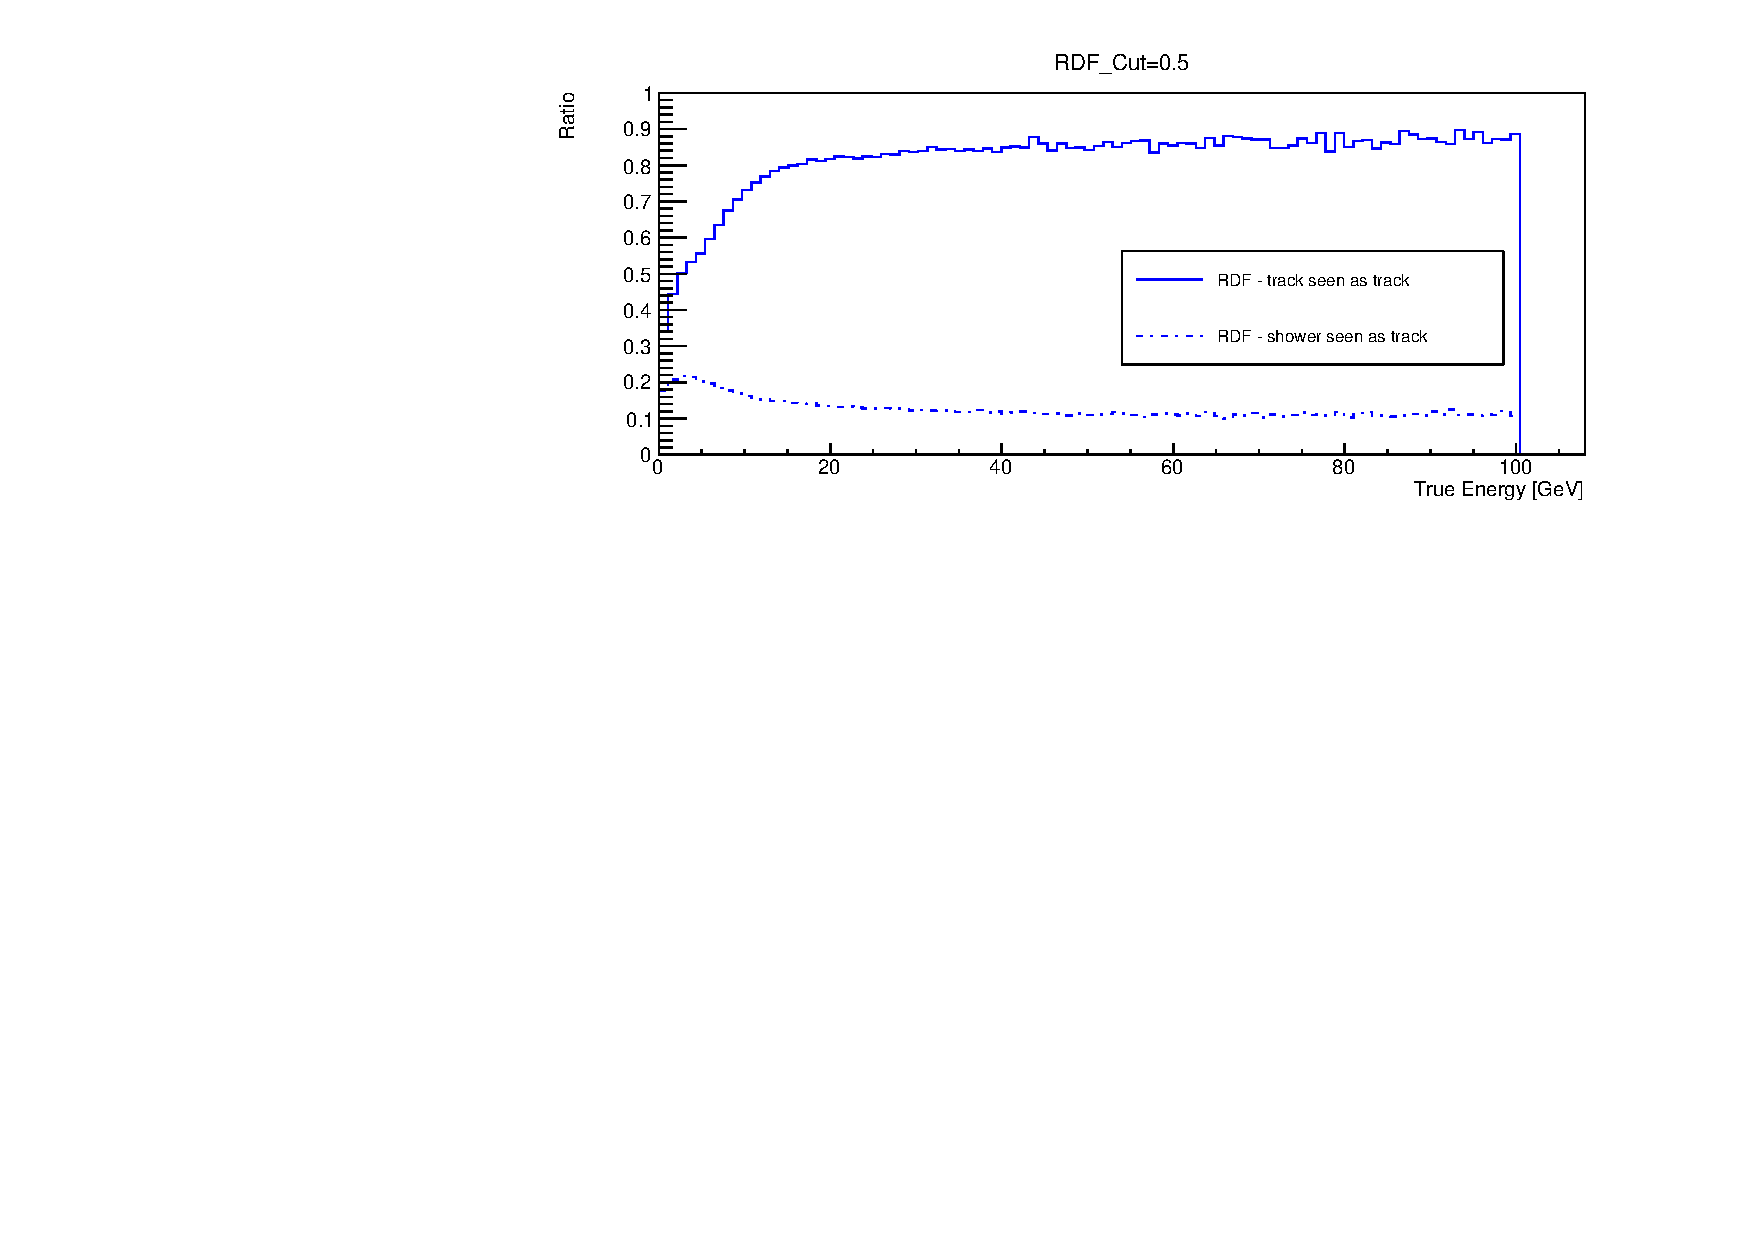
\includegraphics[width=0.9\textwidth]{fig/PID_Efficiency_RDF_CUT_0_5_E_cut_100.pdf}
    \caption{Ratio of track-like events (full line) and shower-like events (dotted line) seen as track, as a function of the true energy --- 0--100 GeV range --- cut = 0.5 --- RDF}
    \label{fig:JYVHJ}
\end{figure}

This plot can be divided into two parts. One above 20 GeV, where the two fractions are constant, and where the classifier performs well: close to 90\% of the track-like events are classified correctly, and no more than 10\% of the shower-like events are incorrectly classified. In the other part, below 20 GeV, the classification gets significantly worse: the fraction of track-like events correctly identified decreases abruptly, and the fraction of incorrectly classified shower-like events slowly increases. Though unfortunate, this trend is not surprising as, the lower the energy of a muon neutrino, the lower the energy of the muon created through a CC muon-neutrino event, and the lower the length of the muon track in the detector. Thus low energy CC muon neutrino events tend to look closer to shower-like events.

\subsection{Purity plot}

\qquad When comparing the results of two different trainings, it is sometimes difficult to tell which training led to a better result, for example when the fraction of events classified as track-like decreases for both classes. Another quantity can be defined for each of the two final classes, "seen as track-like" and "seen as shower-like": the purity, like in Eq. \refeq{EIOZ}, measuring the ratio of correctly classified events in regards to the total number of events classified, in one category.

\begin{equation}
    \left\{
    	\begin{array}{ll}
    		Purity(\text{track-like})=\frac{\text{\large N(track-like\;seen\;as\;track)}}{\text{\large N(track-like\;seen\;as\;track) + N(shower-like\;seen\;as\;track)}} \\[10pt]
		    Purity(\text{shower-like})=\frac{\text{\large N(shower-like\;seen\;as\;shower}}{\text{\large N(track-like\;seen\;as\;shower) + N(shower-like\;seen\;as\;shower)}}
    	\end{array}
   	\right.
    \label{EIOZ}
\end{equation}
where N(class) is the number of events in the class considered.

The purity of each class for the RDF is plotted in Fig. \ref{fig:KJINDE}, again as a function of the true energy of the neutrino, and for a cut on the classifier output at 0.5.

\begin{figure}[h!]
    \centering
    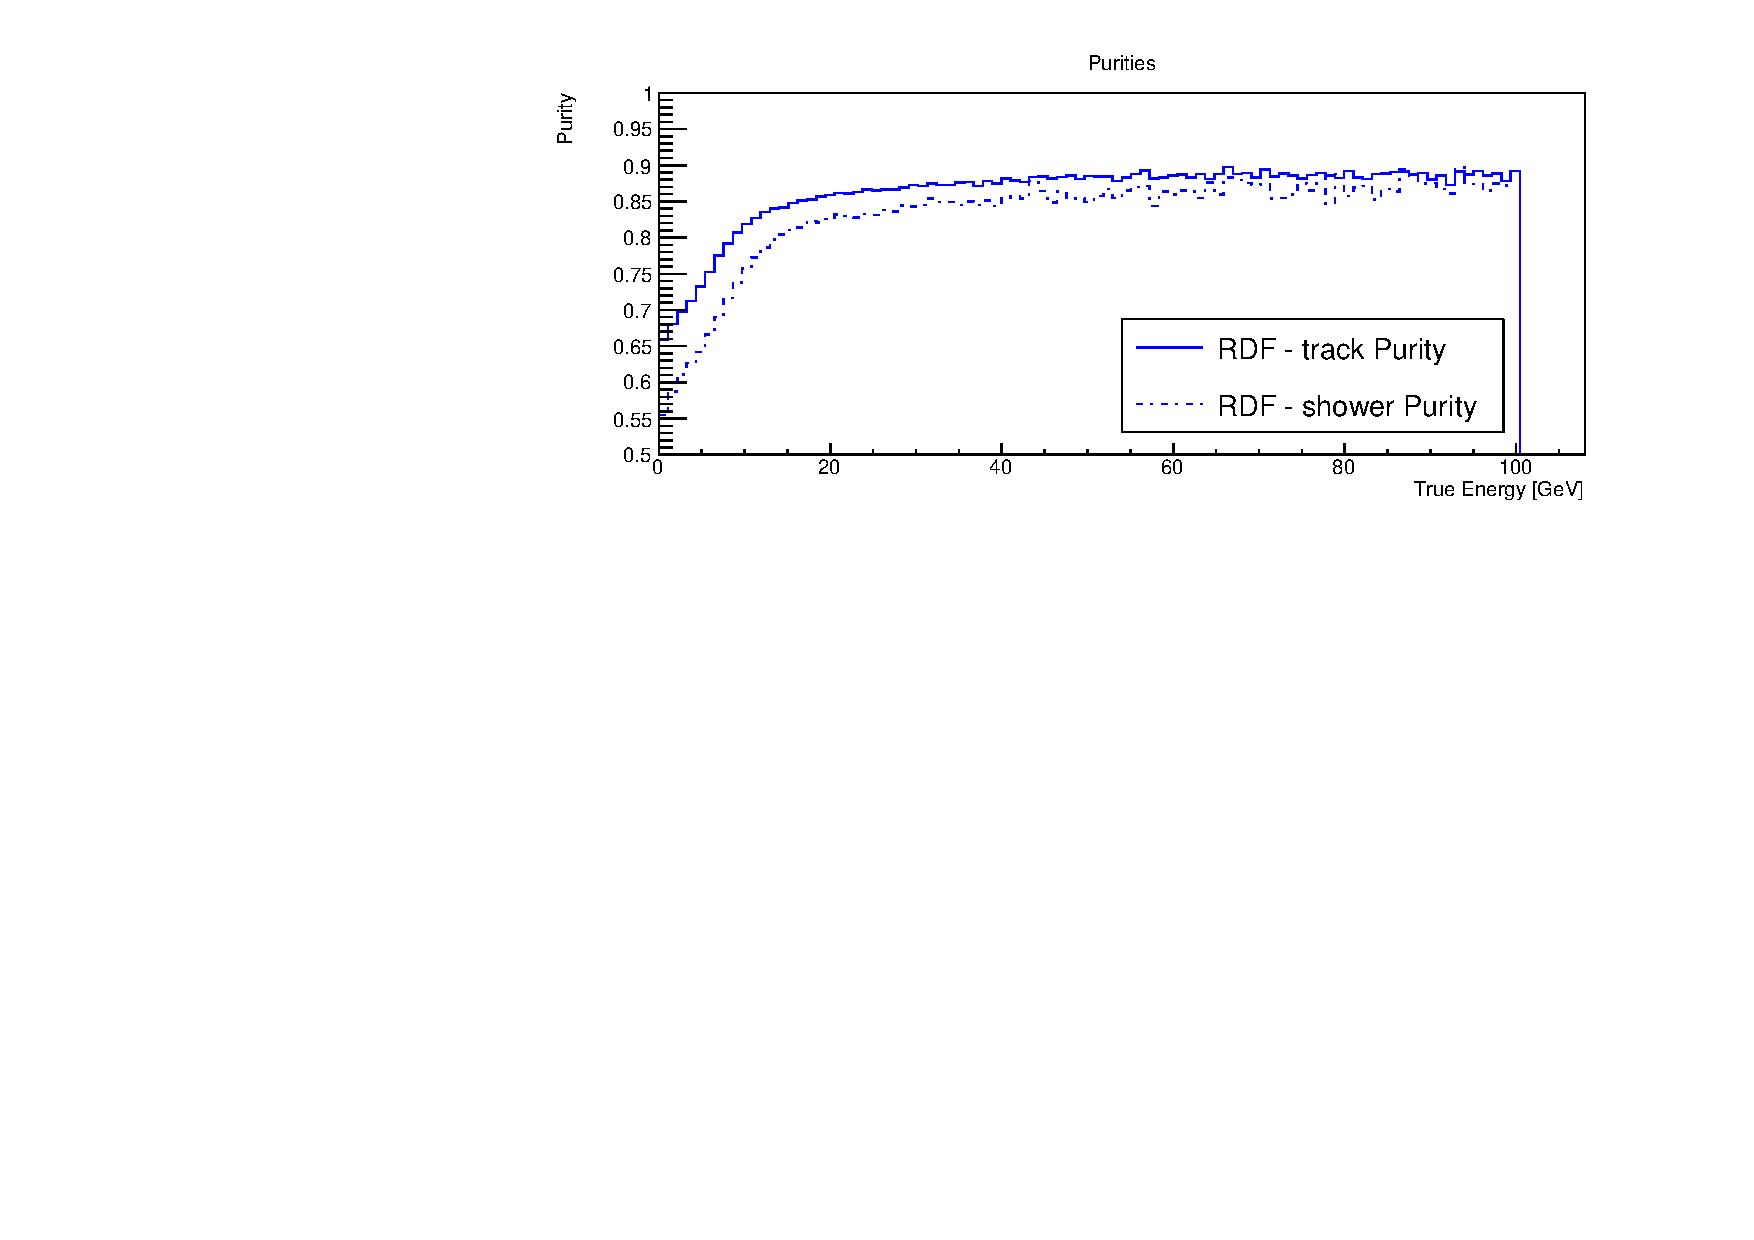
\includegraphics[width=0.9\textwidth]{fig/PID_Purity_RDF_CUT_0_5_E_cut_100.pdf}
    \caption{Purities of the track-like (full lines) and shower-like (dotted lines) classes, as a function of the true energy  --- 0--100 GeV range --- cut = 0.5 --- RDF}
    \label{fig:KJINDE}
\end{figure}

The same two parts can be seen here, with purities relatively constant above 20 GeV, and a drop at low energy, with the seen as shower-like class dropping as low as 55\% purity. Because track-like events tend to be identified as showers at low energies while the proportion of badly classified shower-like events remains rather constant, the purity of the seen as shower class remains lower than the purity of the other class.

The results presented in this section correspond to a cut value on the classifier output of 0.5. What is the influence of the cut value on these efficiencies and on those purities?

\section{Influence of the cut on the classifier output}

\paragraph{} As it has been said in section 1.2.2 the value of the cut will greatly affect the result of the classification. In this study we decided to apply only one cut, and not to discard any event. In Fig. \ref{fig:JHYD}, we can see the effect of the cut on the standard PID plot for the RDF, for the track-like events on the top plot, and the shower-like events on the bottom plot. As the value of the cut increases, both ratio decrease as we can see in Fig. \ref{fig:ABHD}, where the classifier output distribution of the RDF is represented with the cut positioned at 0.5.. As we shift the cut towards 1, we simply ask for events to have more characteristic patterns for the neural network to classify them as track-like ($\hat{y_a}=1$). But as this one class thus increases its purity, the other one's purity gets worse.

\begin{figure}[!h]
    \centering
    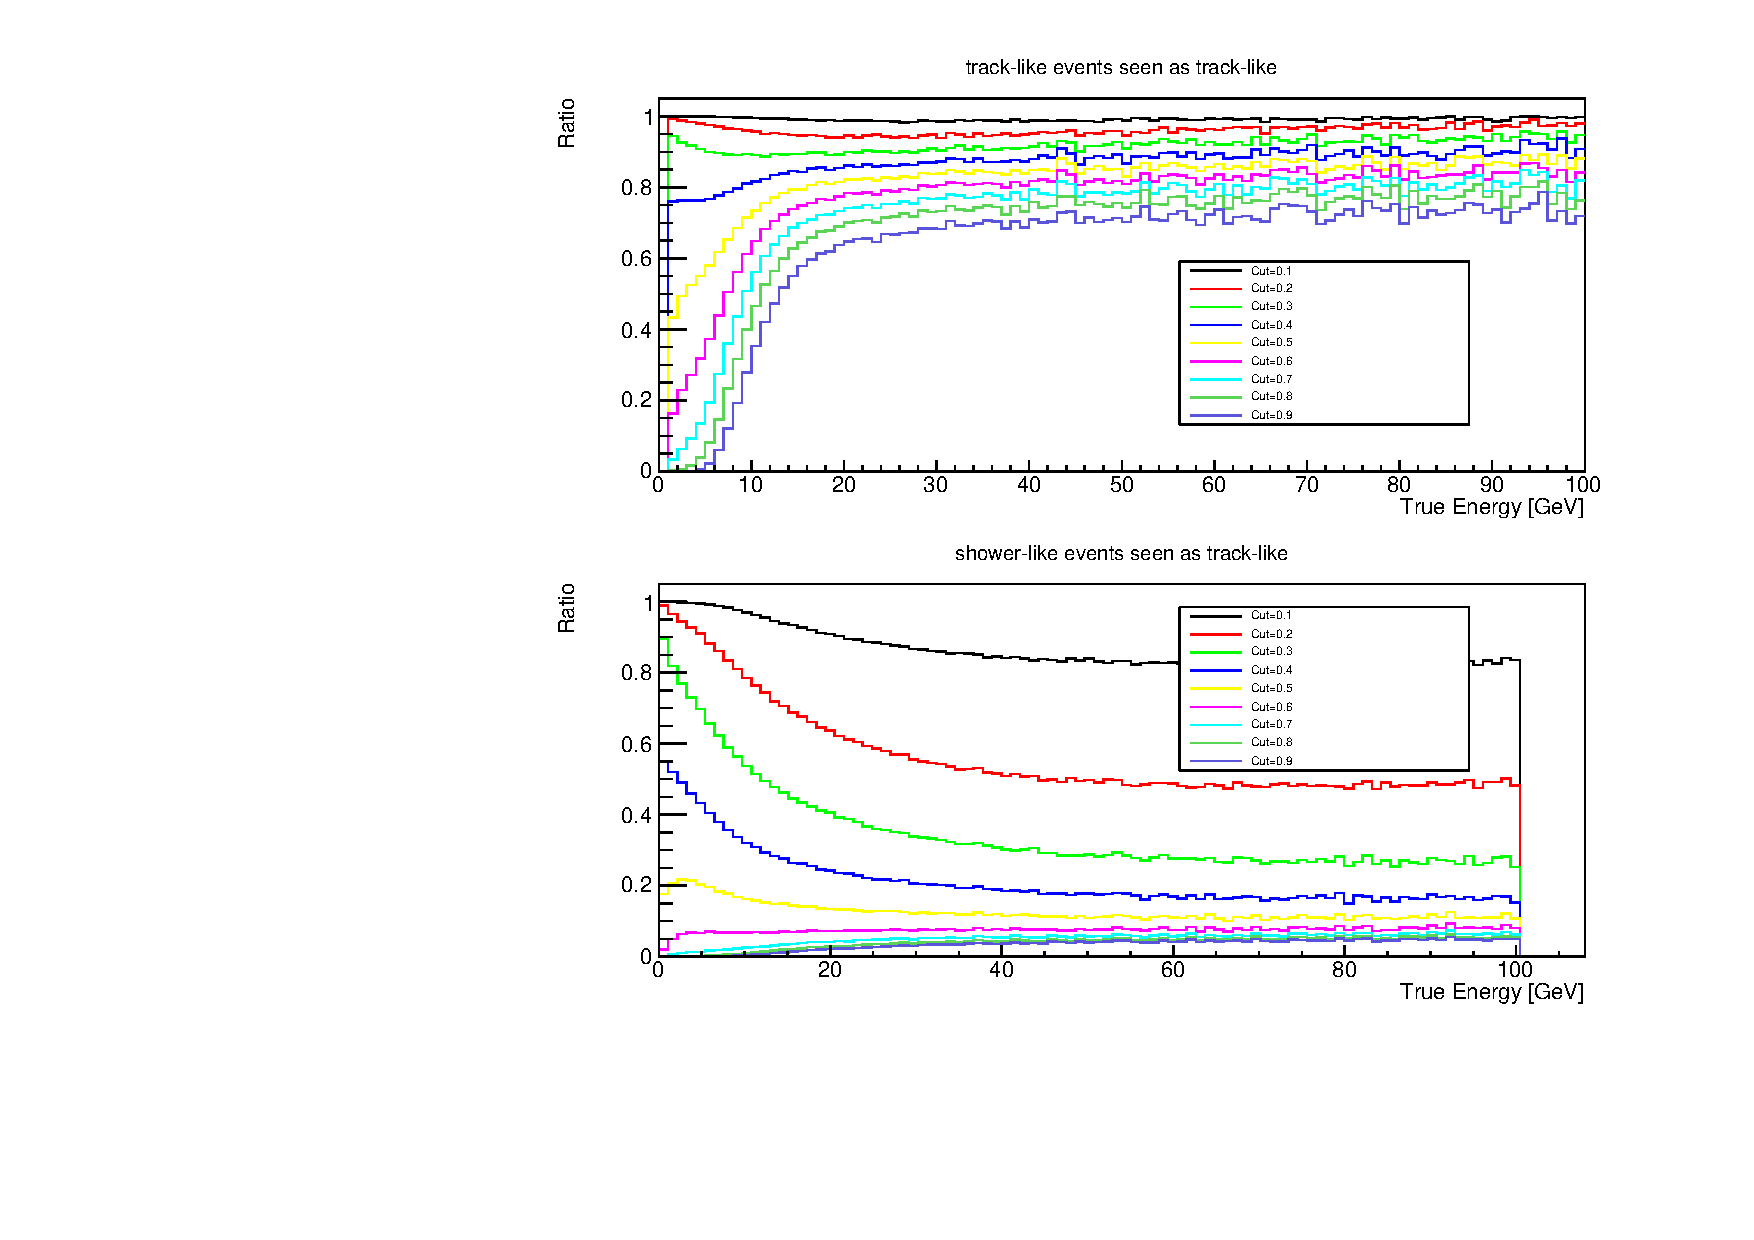
\includegraphics[width=0.9\textwidth]{fig/Cuts_comparison.pdf}
    \caption{Ratio of track-like events (top) and shower-like events (bottom) seen as track, as a function of the true energy, for various values of the classifier cut --- 0--100 GeV range --- RDF}
    \label{fig:JHYD}
\end{figure}

\begin{figure}[!h]
    \centering
    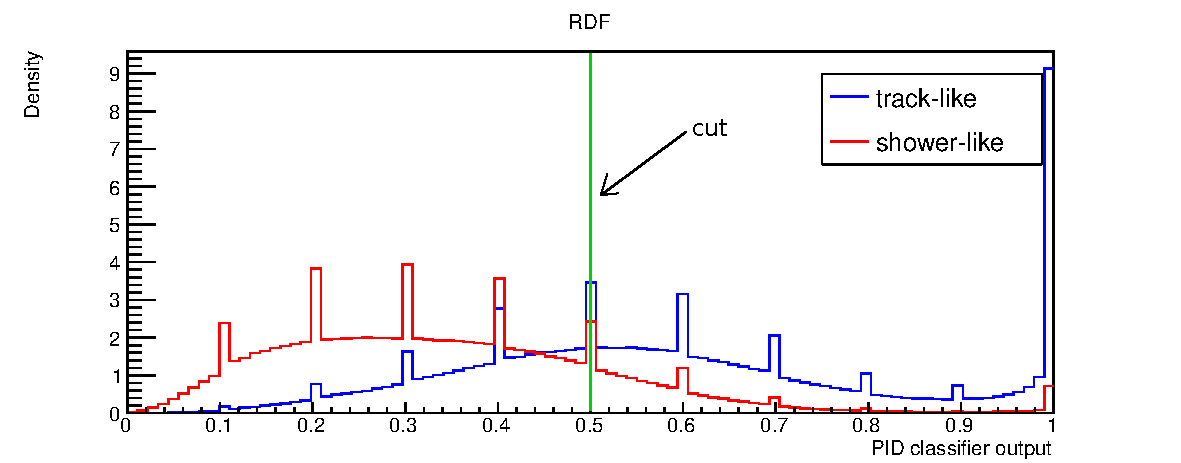
\includegraphics[width=0.9\textwidth]{fig/PID_Classifier_RDF_E_cut_100.pdf}
    \caption{Distributions of the classifier output of the test sample classified by the RDF, for the shower-like events (red) and track-like events (blue). Each distribution is normalised to the total number of events considered. The green line represents the position of the cut.}
    \label{fig:ABHD}
\end{figure}

\paragraph{}
The usual values adopted for the cut remain around 0.5. Such values keep a balance between the purities of the two classes, and the efficiency of the classification for both class. This is no different for the neural network built.

\newpage
\section{Our neural network}

\paragraph{}
The RDF has been trained using all the reconstruction variables available: a number close to two hundred. The neural network, as we said in section 2.1, is only fed thirty variables. The performance of the neural network is compared to the one of the RDF: in Fig. \ref{fig:INLDN} the standard PID plots, and in Fig. \ref{fig:OIDLMRU} the purities of the track-like and and of the shower-like classes. In the two figures, the neural network's performance is shown in red, and the RDF's in blue. The neural network's cut value of 0.6 is chosen so that it matches the RDF performance.

At high energy, the results are similar. The efficiencies are close, the RDF having a better efficiency for the track-like channel while the neural network does better in the shower-like channel. The purities also cannot be used to chose a better classification: the neural network has a better track purity and a worse shower purity, while the RDF sits in the middle for both. However, at low energy the neural network seems to be ahead.

\begin{figure}[!h]
    \centering
    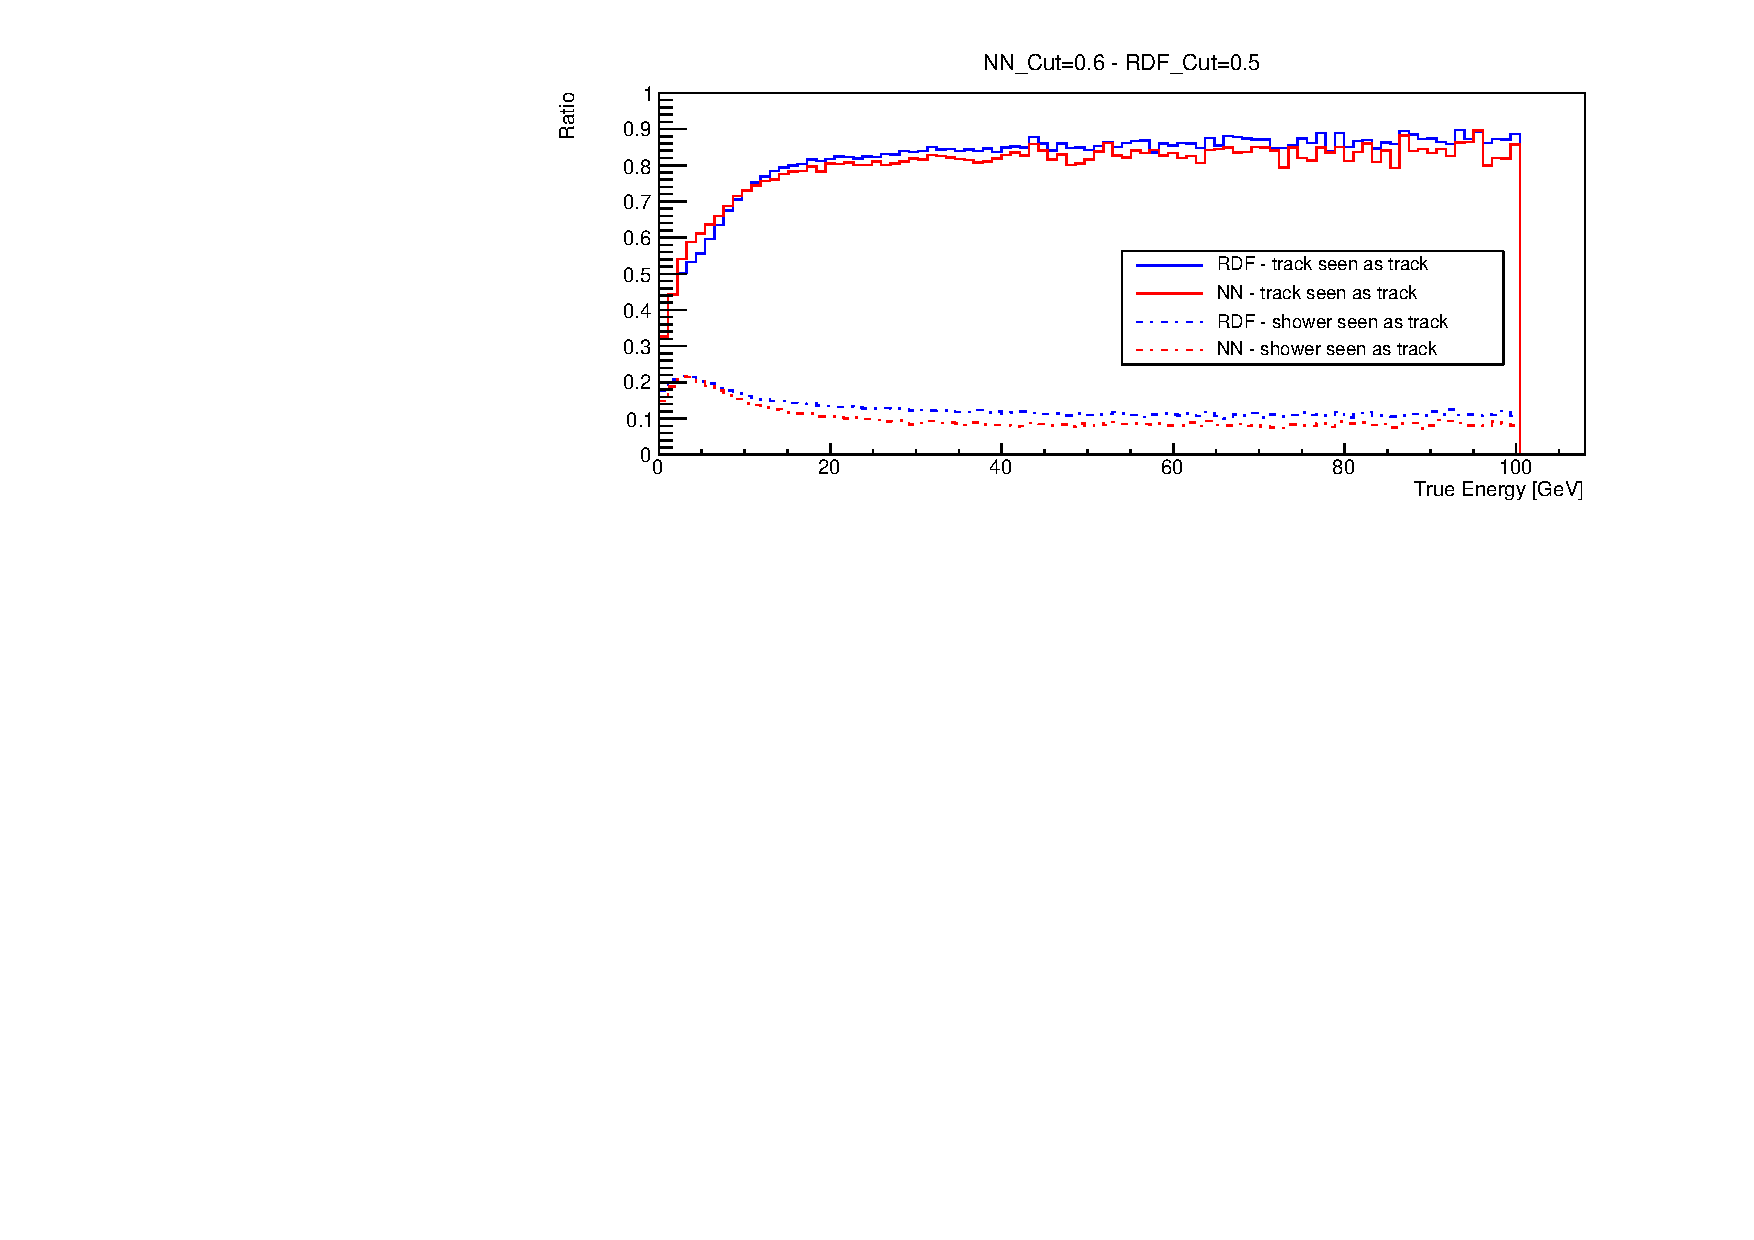
\includegraphics[width=0.9\textwidth]{fig/PID_Efficiency_RDF_CUT_0_5_VS_NN_CUT_0_6_E_cut_100.pdf}
    \caption{Ratio of track-like events (full lines) and shower-like events (dotted lines) seen as track, as a function of the true energy, for the NN (red) and the RDF (blue)  --- 0--100 GeV range --- RDF cut = 0.5 --- NN cut = 0.6}
    \label{fig:INLDN}
\end{figure}

\begin{figure}[!h]
    \centering
    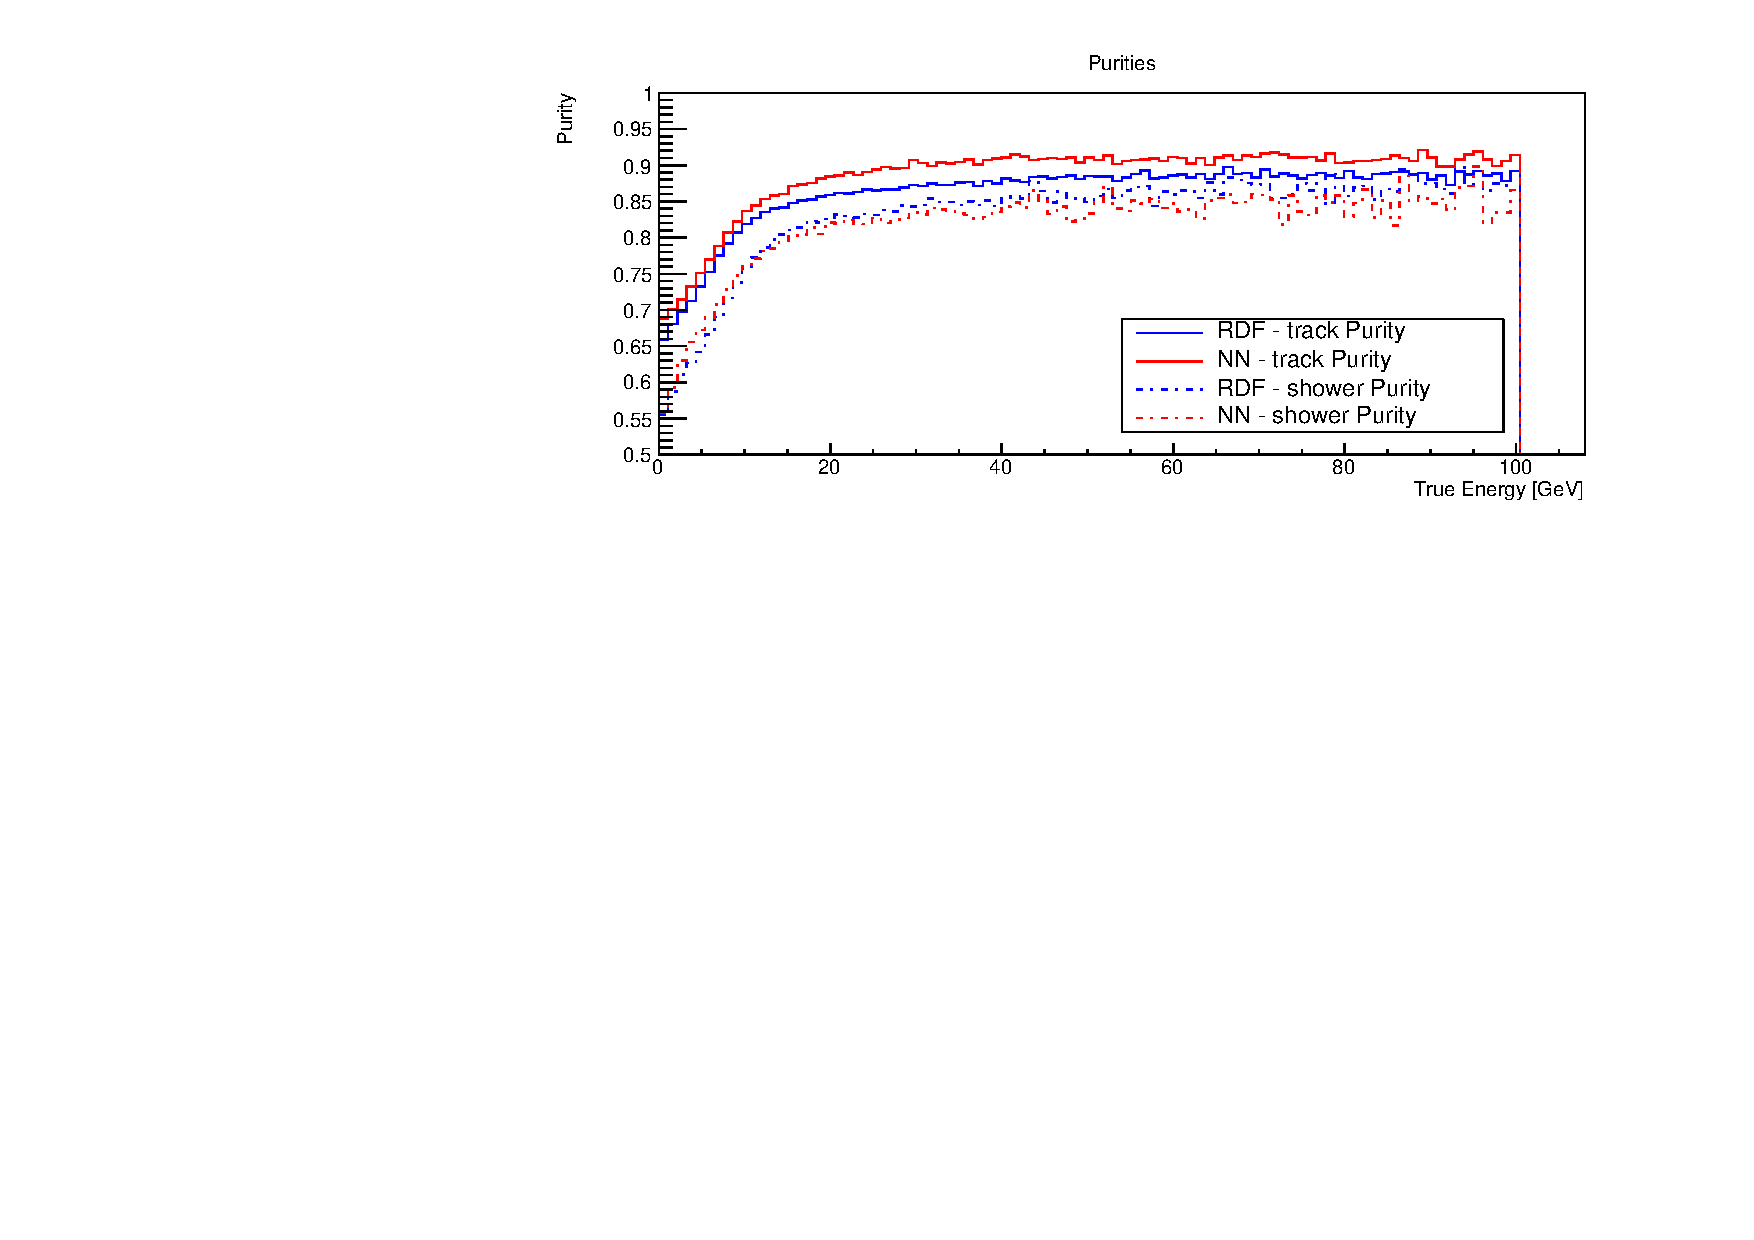
\includegraphics[width=0.9\textwidth]{fig/PID_Purity_RDF_CUT_0_5_VS_NN_CUT_0_6_E_cut_100.pdf}
    \caption{Purities of the track-like (full lines) and shower-like (dotted lines) classes, as a function of the true energy, for the NN (red) and the RDF (blue)  --- 0--100 GeV range --- RDF cut = 0.5 --- NN cut = 0.6}
    \label{fig:OIDLMRU}
\end{figure}

Indeed, a zoom onto the low-energy range shows a clear improvement using the neural network. In Fig. \ref{fig:EUFBKBF}, the standard PID plot is shown for energies in the range 1--20 GeV, witht the same colour code as previously. The neural network has a lower ratio of incorrectly classified shower-like events in the whole range, and the ratio of correctly classified track-like events stays close to the one of the RDF for most of the energy range, except around 4 GeV where the neural network see the best improvement. The purity plot in Fig. \ref{fig:SLKNPE} shows the neural network ahead in the whole 1--20 GeV energy range, in terms of purity, which amply compensates for the slight loss of efficiency. As we are interested in the 1--10 GeV range, this is an interesting result.

\begin{figure}[!h]
    \centering
    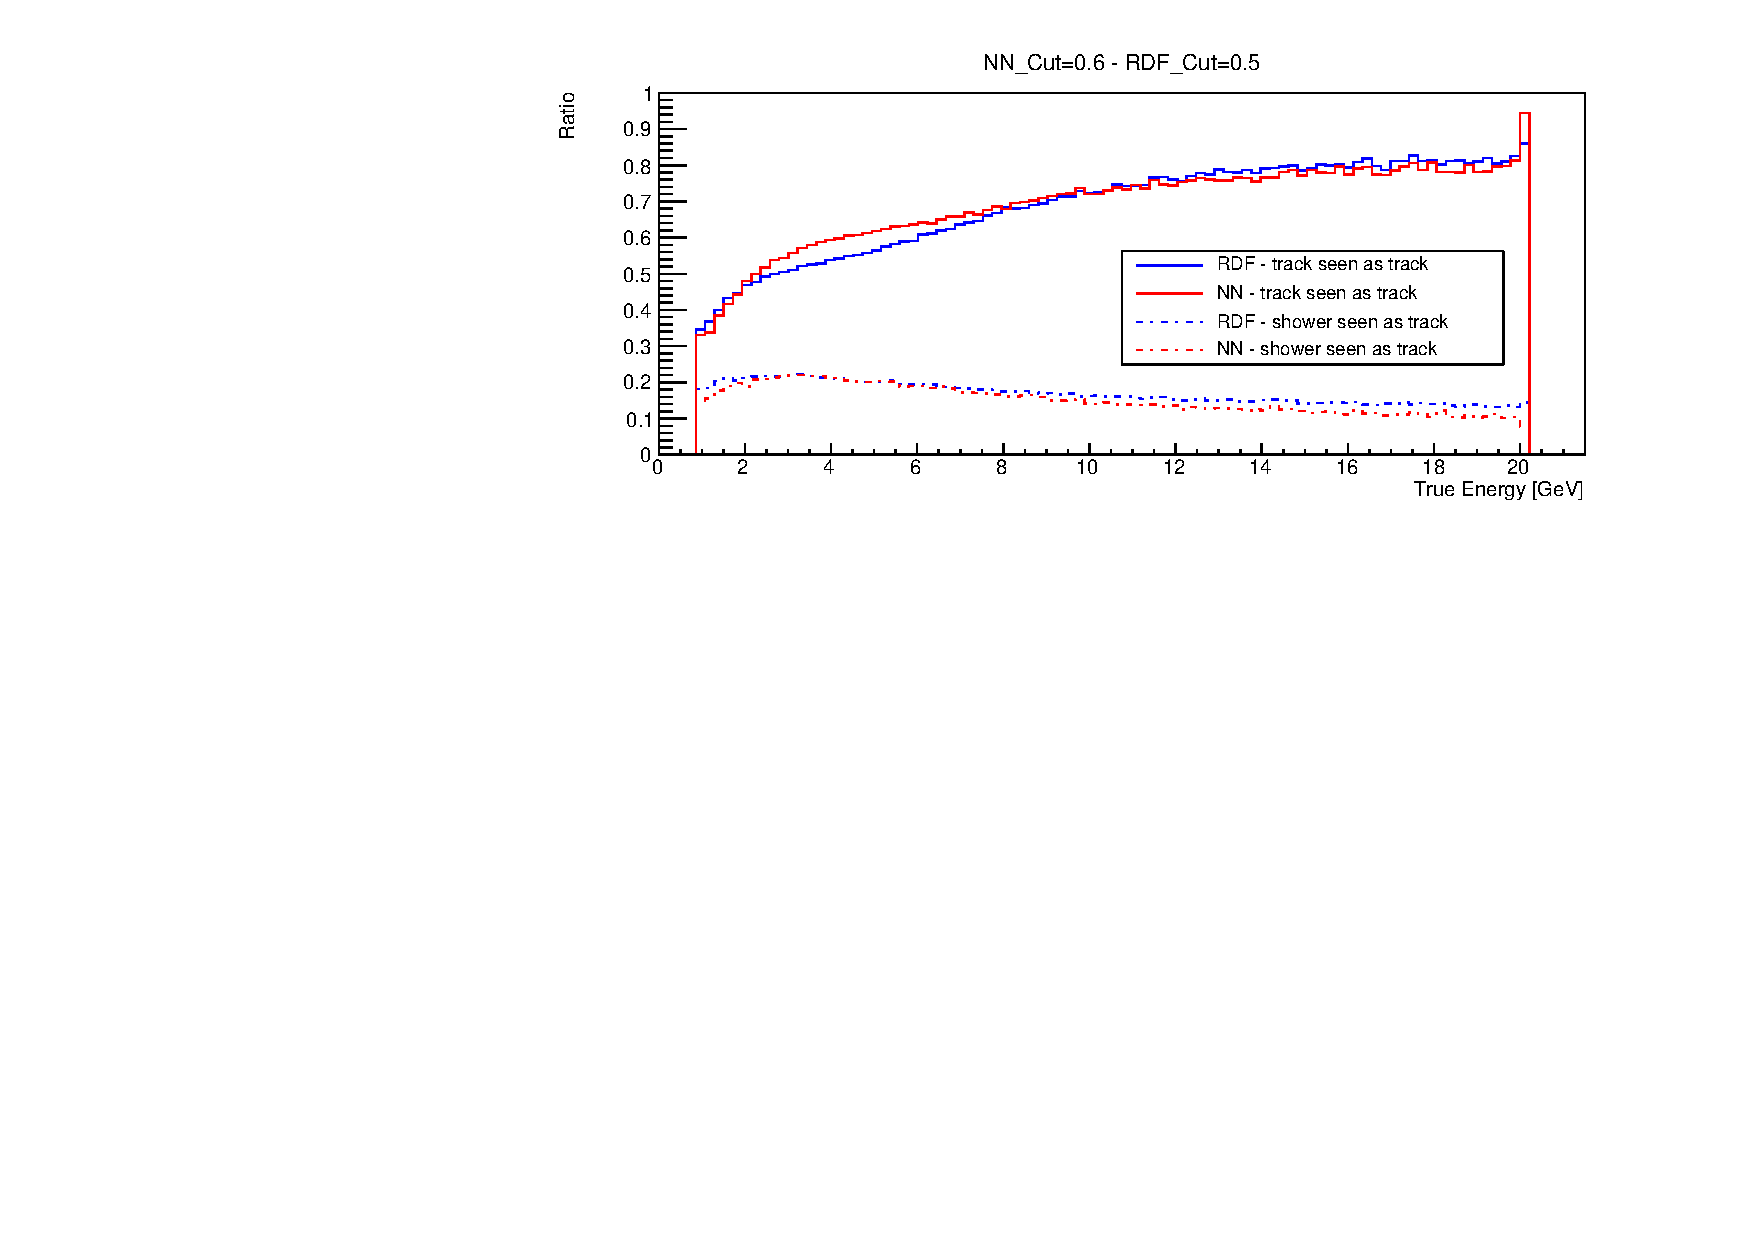
\includegraphics[width=0.9\textwidth]{fig/PID_Efficiency_RDF_CUT_0_5_VS_NN_CUT_0_6_E_cut_20.pdf}
    \caption{Ratio of track-like events (full lines) and shower-like events (dotted lines) seen as track, as a function of the true energy, for the NN (red) and the RDF (blue)  --- 0--20 GeV range --- RDF cut = 0.5 --- NN cut = 0.6}
    \label{fig:EUFBKBF}
\end{figure}

\begin{figure}[!h]
    \centering
    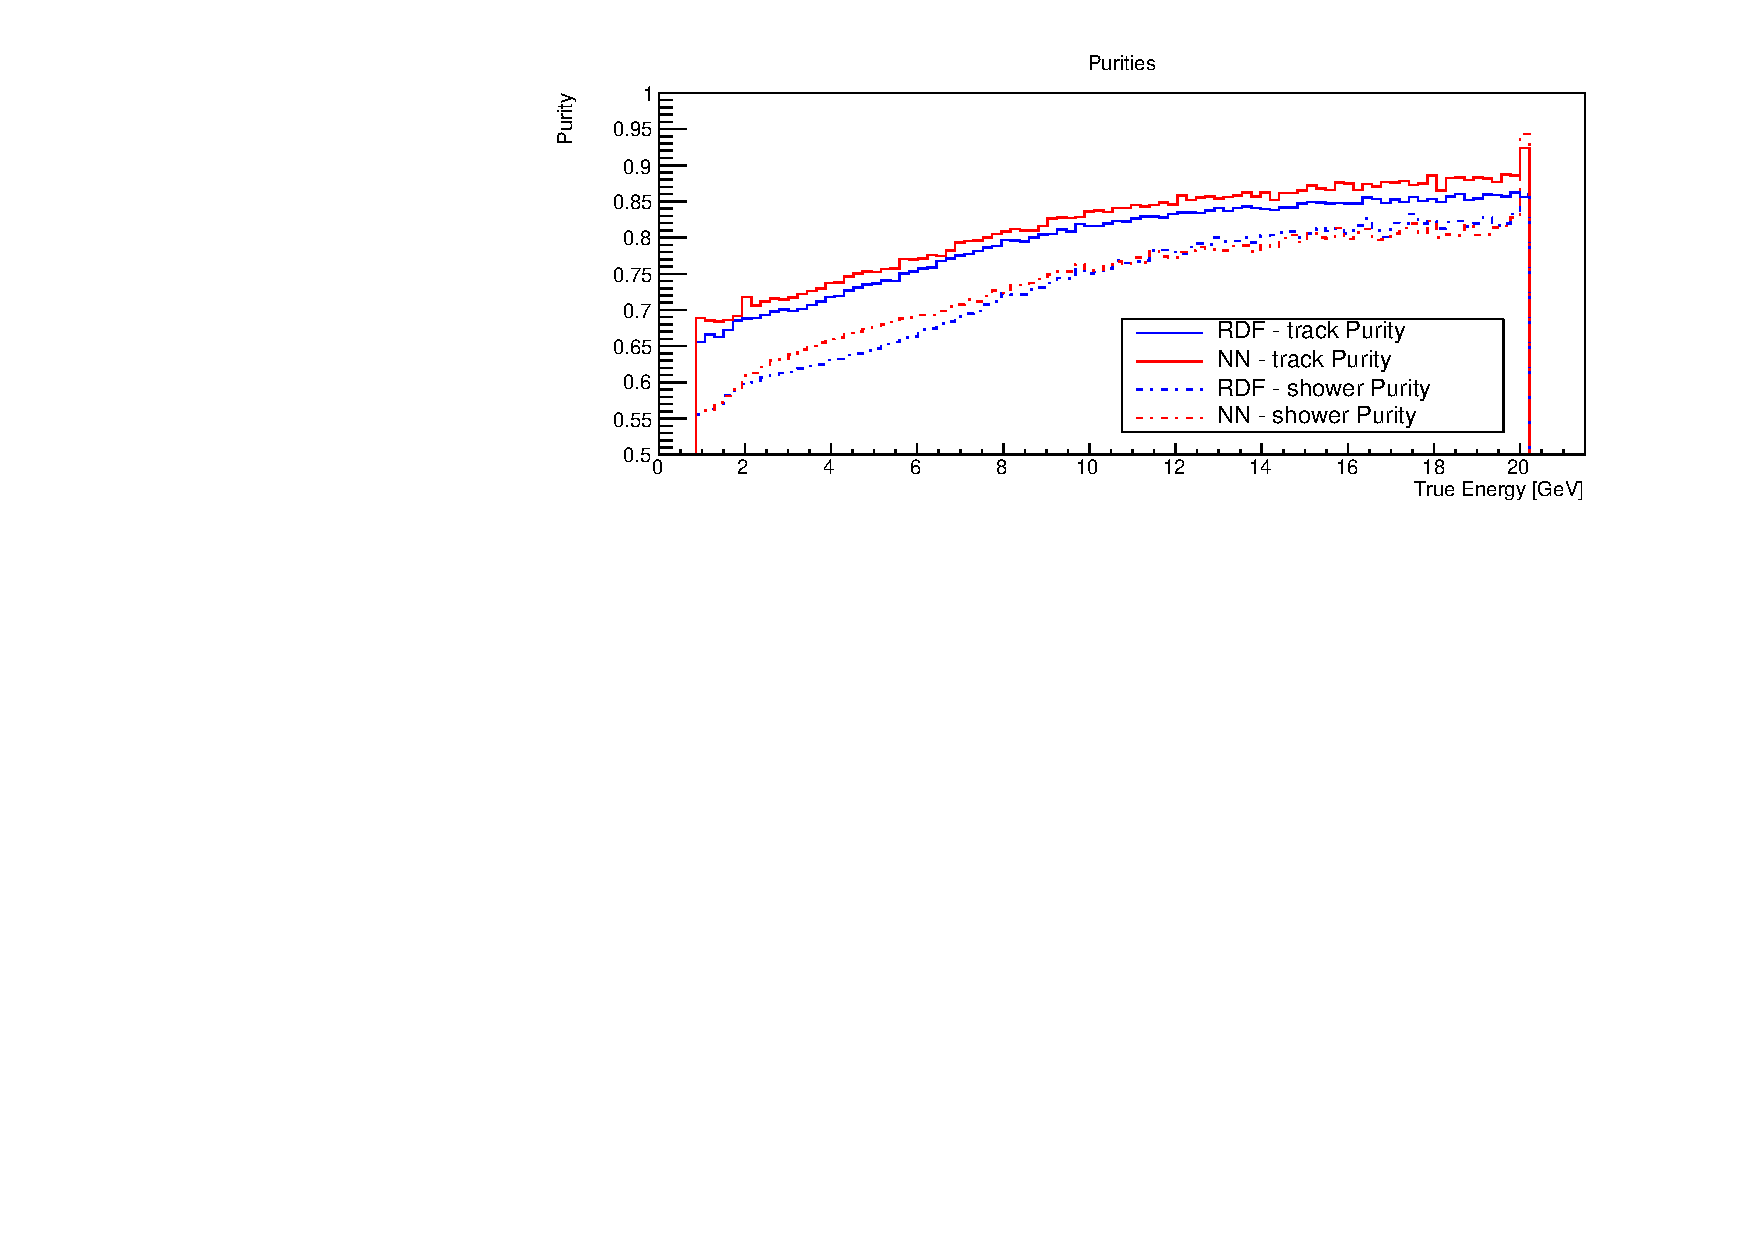
\includegraphics[width=0.9\textwidth]{fig/PID_Purity_RDF_CUT_0_5_VS_NN_CUT_0_6_E_cut_20.pdf}
    \caption{Purities of the track-like (full lines) and shower-like (dotted lines) classes, as a function of the true energy, for the NN (red) and the RDF (blue)  --- 0--20 GeV range --- RDF cut = 0.5 --- NN cut = 0.6}
    \label{fig:SLKNPE}
\end{figure}

This neural network validates two of the objectives set at the beginning of this study. First its classification at low energies outperforms the one of the Random Decision Forest, and although the absolute gain shown in the efficiency plots is slight, the relative improvement as seen in the purity plots is not negligible. Besides that, this neural network only uses thirty variables, much less than the close-to-two-hundred variables needed for the Random Decision Forest.

\chapter*{Conclusion}
\addcontentsline{toc}{chapter}{Conclusion}

The objective of this work was to improve the particle identification at the energy-range 1--10 GeV, and to reduce the number of variables used in the classification. The first part of this report presented the NMH problem and how KM3NeT/ORCA plans to solve it, and introduced the tools necessary to the PID. The second part detailed the construction of the neural network used in this work as well as the quantities that would then be used to compare the performance of this same neural network with the one of the RDF. The conclusion is that both objectives have been reached, as the neural network both outperforms the Random Decision Forest and uses less variables than it.

There is still a lot of room for improvement: obviously all the combinations of variables have not been studied, and selecting variables solely on their individual performance, as we did in this study, does leave a lot of good possible candidates out: indeed, a neural network extract the information from the whole multi-dimensional space we feed it, and can thus see correlations between variables that can help for the classification. However, testing all the possible pools of variables would necessitate a lot of computing power, as just one set of 30 variables takes around 24 hours for the neural network to train on the machines used during this work. Another approach should be found.




\bibliography{main}
\addcontentsline{toc}{chapter}{Bibliography}
\nocite{*}
\bibliographystyle{apa} 


\chapter*{Abstract}

Most of the parameters governing the neutrino oscillations have been measured in the last decades. One of the remaining unknowns is the question of the Neutrino Mass Hierarchy. Answering this question is one of the main missions of the KM3NeT/ORCA detector. One of the critical steps in the NMH measurement is the identification of the flavour of the detected neutrinos. If the current tools used to discriminate between the different flavours -- a machine learning algorithm called Random Decision Forest -- performs well at the high-end of the energy range seen by KM3NeT/ORCA, the performance achieved at the lower edge (1--10 GeV) is relatively poor. Besides, this algorithm use brute force to classify the events by using all of the near two hundred variables reconstructed from the raw data of the detector. The goal of this study is to improve the particle identification at these energies by using a different kind of machine learning algorithm -- a Neural Network -- and to reduce the number of variables necessary to the classification. After introducing the background and tools necessary to the understanding of the study, the performance of the neural network built is compared to the one of the Random Decision Forest already in use. It appears that both objectives are met by the new neural network.

{\let\clearpage\relax \chapter*{Résumé}}

La plupart des paramètres gouvernant les oscillations des neutrinos ont été mesurés durant les dernières décennies. Une question ouverte qui subsiste est la question de la Hiérarchie de Masse des Neutrinos. Celle-ci est une des missions principales du détecteur KM3NeT/ORCA. Une des étapes critiques à la détermination de cette hiérarchie est l'identification de la saveur des neutrinos détectés. Si l'outil utilisé aujourd'hui, un algorithme d'apprentissage automatique appelé Forêt d'Arbres Décisionnels, montre de bonnes performances dans la partie haute du spectre d'énergie des neutrinos détectés par KM3NeT/ORCA, la partie inférieure de ce spectre (1--10 GeV) voit de plutôt faibles performances. En plus de cela, cet algorithme utilise la force brute pour discriminer les évènements en utilisant toutes les quelques deux-cent variables reconstruites à partir des données brutes du détecteur. L'objectif de cette étude est d'améliorer les capacités de discrimination aux basses énergies en utilisant un autre type d'algorithme d'apprentissage automatique, un réseau de neuronnes, et de réduire le nombre de variables nécessaires à la classification. Après avoir introduit les notions et outils nécessaires à la compréhension de cette étude, les performances du réseau de neuronnes construit sont comparées à celles de la Forêt d'Arbres Décisionnels utilisée jusque là. Il apparaît que les deux objectifs sont atteints par le nouveau réseau de neuronnes.

\thispagestyle{empty}


\end{document}
